\documentclass{beamer}

\title{B-Trees}
\author{%
    Martín Hernández\\%
    Juan Mendivelso%
}
\date{} % Empty Date

% Libraries / Packages
\usepackage{graphicx} % Required for inserting images
\usepackage{geometry}
    \geometry{paperwidth=8in,paperheight=5in}
\usepackage{tcolorbox}
\usepackage{mathtools}
\usepackage{unicode-math}
\usepackage{listings}
\usepackage{luacolor}
\usepackage{lua-ul}
\usepackage{minted}
\usepackage{enumitem}
\usepackage{csquotes}
\usepackage{booktabs}
\usepackage{biblatex}
    \addbibresource{resources/bibliography.bib}

\setlist[itemize]{label=>}

\NewDocumentCommand{\examplefnt}{}{\fontsize{7.5pt}{8pt}\selectfont}
\definecolor{lightCyan}{Hsb}{195, 0.35, 1}
\LuaULSetHighLightColor{lightCyan}
\NewDocumentCommand{\hlght}{m}{%
    \highLight{#1}%
}

\NewDocumentCommand{\rarr}{}{\(\rightarrow\)}

% Template
\NewDocumentCommand{\shortauthors}{}{%
    Hernández, %
    Mendivelso%
}
% Listings code env and inline stuff
\lstset{%
basicstyle=\ttfamily%
}

\lstdefinestyle{codeinc}{%
    escapechar=\%,%
    numbers=left,%
    stepnumber=1,%
    tabsize=1,%
    commentstyle=\color{gray},%
    basicstyle=\small,%
    breaklines=true,%
    language=C%
}

% Text
\setbeamercolor{titlelike}{fg=black}
\setbeamerfont{titlelike}{size=\Large,series=\bfseries}

\setbeamerfont{title}{series=\bfseries,size=\huge}
\setbeamerfont{structure}{series=\bfseries,size=\large}
\setbeamercolor{structure}{fg=black}

\setbeamercolor{footline}{fg=gray}
\setbeamerfont{footline}{size*={4.5}{-1}}
\setbeamerfont{framenumber}{size*={8}{0}}

% Frame columns sizes

\newcommand{\textlecolumn}{0.9\textwidth}
\newcommand{\textricolumn}{0.1\textwidth}

% Footline
\setbeamertemplate{navigation symbols}{}
\setbeamertemplate{footline}{%
    \hbox{%
        \begin{beamercolorbox}[wd=1\paperwidth,dp=2.5ex,right]{framenumber}%
            \usebeamerfont{framenumber}
            \insertframenumber{}%
            \hspace*{2ex}%
        \end{beamercolorbox}
    }%
    \vskip0pt%
    %
    \begin{center}%
        \vspace{-4mm}
        Presentation made by \shortauthors{}. Contents and figures extracted from the book: Advanced Data Structures. Peter Brass. Cambridge University Press. 2008.
        \vspace{-3mm}
    \end{center}%
%
}

\begin{document}
% Code elemenst definitions
\defverbatim[colored] \btreeStructure {%
\begin{lstlisting}[style=codeinc]
int alpha = 2 /* any int >= 2 */
typedef struct tr_n_t {
  int degree;
  int height;
  key_t key[2 * alpha];
  struct tr_n_t * next[(2 * alpha) + 1];
  /* possibly other information */
} tree_node_t;
\end{lstlisting}
}

\defverbatim[colored] \btreeCreateEmpty {%
\begin{lstlisting}[style=codeinc]
tree_node_t *create_tree(){ 
  tree_node_t *tmp;
  tmp = get_node();
  tmp->height = 0;
  tmp->degree = 0;
  return( tmp );
}
\end{lstlisting}
}

\defverbatim[colored] \btreeSearch {%
\begin{lstlisting}[style=codeinc]
object_t *find(tree_node_t *tree, key_t query_key) { 
  tree_node_t *current_node;
  object_t *object;
  current_node = tree;
  while( current_node->height >= 0 ) { /* binary search among keys */
    int lower, upper;
    lower = 0;
    upper = current_node->degree;
    while( upper > lower +1 ) {
      if( query_key < current_node->key[(upper+lower)/2 ] )
        upper = (upper+lower)/2;
      else
        lower = (upper+lower)/2;
    }
    if( current_node->height > 0)
      current_node = current_node->next[lower + 1]; /* Offset sub-tree ptrs def */
    else { /* block of height 0, contains the object pointers */
      if( current_node->key[lower] == query_key )
        object = (object_t *)
        current_node->next[lower];
      else
        object = NULL;
      return( object );
    }
  }
}
\end{lstlisting}
}

\defverbatim[colored] \btreeDestroy {%
\begin{lstlisting}[style=codeinc]
void btDestroy(bTree b) {
  if(!b->isLeaf) {
    for (int i = 0; i < b->numKeys + 1; i++) {
      btDestroy(b->kids[i]);
    }
  }
  free(b);
}
\end{lstlisting}
}

\defverbatim[colored] \btreeSearchStepOne {%
\begin{lstlisting}[style=codeinc,numbers=none]
query_key = 16;
tree = *(node 1);

object = NULL;
current_node = *(node 1);
current_node->height = 1;
current_node->degree = 2;

lower = 0;
upper = 2;
\end{lstlisting}
}

\defverbatim[colored] \btreeSearchStepTwo {%
\begin{lstlisting}[style=codeinc,numbers=none]
query_key = 16;
tree = *(node 1);

object = NULL;
current_node = *(node 1);
current_node->height = 1;
current_node->degree = 2;

lower = 2; 
upper = 2;
\end{lstlisting}
}

\defverbatim[colored] \btreeSearchStepThree {%
\begin{lstlisting}[style=codeinc,numbers=none]
query_key = 16;
tree = *(node 1);

object = NULL;
current_node = *(node 5);
current_node->height = 0;
current_node->degree = 3;

lower = 0; 
upper = 3;
\end{lstlisting}
}

\defverbatim[colored] \btreeSearchStepFour {%
\begin{lstlisting}[style=codeinc,numbers=none]
query_key = 16;
tree = *(node 1);

object = NULL;
current_node = *(node 5);
current_node->height = 0;
current_node->degree = 3;

lower = 0; 
upper = 2;
\end{lstlisting}
}

\defverbatim[colored] \btreeSearchStepFive {%
\begin{lstlisting}[style=codeinc,numbers=none]
query_key = 16;
tree = *(node 1);

object = NULL;
current_node = *(node 5);
current_node->height = 0;
current_node->degree = 3;

lower = 0; 
upper = 1;
\end{lstlisting}
}

\defverbatim[colored] \btreeSearchStepSix {%
\begin{lstlisting}[style=codeinc,numbers=none]
query_key = 16;
tree = *(node 1);

object = *(16);
current_node = *(node 5);
current_node->height = 0;
current_node->degree = 3;
\end{lstlisting}
}

\defverbatim[colored] \btreeSearchStepSeven {%
\begin{lstlisting}[style=codeinc,numbers=none]
query_key = 16;
tree = *(node 1);

object = NULL;
current_node = *(node 5);
current_node->height = 0;
current_node->degree = 3;
\end{lstlisting}
}

\defverbatim[colored] \btreeInsert {%
\begin{lstlisting}[style=codeinc]
void btInsert(bTree b, int key) {
  bTree b1, b2;
  int median;

  b2 = btInsertInternal(b, key, &median);
  if(!b2) {
    return;
  }
  
  b1 = malloc(sizeof(*b1));
  memmove(b1, b, sizeof(*b));
  b->numKeys = 1;
  b->isLeaf = 0;
  b->keys[0] = median;
  b->kids[0] = b1;
  b->kids[1] = b2;
}
\end{lstlisting}
}

\defverbatim[colored] \btreeInsertInternalPartOne {%
\begin{lstlisting}[style=codeinc]
bTree btInsertInternal(bTree b, int key, int *median) {
  int pos = searchKey(b->numKeys, b->keys, key);
  int mid;
  bTree b2;

  if(pos < b->numKeys && b->keys[pos] == key)
    return 0; /* nothing to do */

  if(b->isLeaf) { 
      memmove(&b->keys[pos+1], &b->keys[pos], sizeof(*(b->keys)) * (b->numKeys - pos));
      b->keys[pos] = key;
      b->numKeys++;
  } else {
    ...
\end{lstlisting}
}

\defverbatim[colored] \btreeInsertInternalPartTwo {%
\begin{lstlisting}[style=codeinc,firstnumber=12]
    ...
  } else {
    b2 = btInsertInternal(b->kids[pos], key, &mid);      
    if(b2) {
      memmove(&b->keys[pos+1], &b->keys[pos], sizeof(*(b->keys)) * (b->numKeys - pos));
      memmove(&b->kids[pos+2], &b->kids[pos+1], sizeof(*(b->keys)) * (b->numKeys - pos));

      b->keys[pos] = mid;
      b->kids[pos+1] = b2;
      b->numKeys++;
    }
  }
\end{lstlisting}
}

\defverbatim[colored] \btreeInsertInternalPartThree {%
\begin{lstlisting}[style=codeinc,firstnumber=24]
  ...
  if(b->numKeys >= (2*alpha - 1)) {
    mid = b->numKeys/2;

    *median = b->keys[mid];

    /* make a new node for keys > median */
    b2 = malloc(sizeof(*b2));

    b2->numKeys = b->numKeys - mid - 1;
    b2->isLeaf = b->isLeaf;

    memmove(b2->keys, &b->keys[mid+1], sizeof(*(b->keys)) * b2->numKeys);
    if(!b->isLeaf) {
        memmove(b2->kids, &b->kids[mid+1], sizeof(*(b->kids)) * (b2->numKeys + 1));
    }

    b->numKeys = mid;
    return b2;  
  } else {
    return 0;
  }
}
\end{lstlisting}
}


\begin{frame}
    \titlepage
\end{frame}

\begin{frame}[allowframebreaks,allowdisplaybreaks]
    \frametitle{Contents}
    \tableofcontents
\end{frame}

\begin{frame}[allowframebreaks,allowdisplaybreaks]
    \section{B-Tree}
    \subsection{History}
    \frametitle{B-Tree History}
    \begin{columns}
        \begin{column}{0.5\textwidth}
            \begin{block}{}
                B-Trees where firstly studied, defined and implemented by R. Bayer and E. McCreight in 1972, using an IBM 360 series model 44 with an 2311 disk drive.
                \begin{figure}
                    \centering
                    \includegraphics[width=0.5\textwidth,height=\textheight,keepaspectratio]{resources/made/ibm360_44.png}
                    \caption[]{IBM 360 / 44}
                \end{figure}
            \end{block}
        \end{column}
        \begin{column}{0.5\textwidth}
            \begin{block}{}
                An IBM 360 series model 44 had from 32 to 256 \(KB\) of Random Access Memory, and weighed from 1,315 to 1,905 kg.
                \begin{figure}
                    \centering
                    \includegraphics[width=0.5\textwidth,height=\textheight,keepaspectratio]{resources/made/ibmdisk_2311.png}
                    \caption[]{IBM 2311 disk drive}
                \end{figure}
            \end{block}
        \end{column}
    \end{columns}

    \framebreak

    \begin{columns}
        \begin{column}{0.7\textwidth}
            \begin{block}{}
                \blockquote[Bayer and McCreight]{%
                    (\ldots) actual experiments show that it is possible 
                    to maintain an index of size 15.000 with an average of 9 retrievals, 
                    insertions, and deletions per second in real time on an IBM 360/44 
                    with a 2311 disc as backup store. (\ldots) it should be possible 
                    to main tain all index of size 1'500.000 with at least two transactions 
                    per second.}
            \end{block}
            \begin{block}{}
                \blockquote[Bayer]{%
                    I am occasionally asked what the B in B-Tree means. (\ldots)
                    We wanted the name to be short, quick to type, easy to remember.
                    It honored our employer, Boeing Airplane Company, but we wouldn't have to request permission to use the name.
                    It suggested Balance. Rudolf Bayer was the senior researcher of the two of us. (\ldots)
                    I don't recall one meaning standing out above the others that day. 
                    Rudolf is fond of saying that the more you think about what the B could mean, the more you learn about B-Trees, and that is good.
                }
            \end{block}
        \end{column}
        \begin{column}{0.3\textwidth}
            \begin{block}{}
                \begin{figure}
                    \includegraphics[height=0.3\textheight]{resources/made/r_bayer.png}
                    \caption[]{Rudolf Bayer}
                \end{figure}
                \begin{figure}
                    \includegraphics[height=0.35\textheight]{resources/made/McCreight.png}
                    \caption[]{Edward McCreight}
                \end{figure}
            \end{block}
        \end{column}
    \end{columns}
\end{frame}


\begin{frame}[allowframebreaks,allowdisplaybreaks]
    \subsection{Definition}
    \frametitle{B-Tree Definition}
    \begin{columns}
        \begin{column}{\textlecolumn}
            \begin{block}{}
                \begin{itemize}
                    \item We will define that \(T\), an object, is a B-Tree if they are an instance of the class.
                    \[
                        T \in t\left(\alpha, h\right)
                    \]
                    \item Where \(h\) is the height of the B-Tree.
                    \item And, \(\alpha\) is a predefined constant.
                    \item This type of balanced tree have a higher degree than the previous trees.
                    \item Or in simple words, they have more than 1 key and 2 sub-trees in each node.
                    \item Keep in mind that in B-Trees, \textbf{leafs are not nodes}.
                    \item This higher degree have a cuple of properties added to it, which we need to check and prove
                    \item Also, due to the higher degree of the nodes, we will have to change the 
                        \lstinline|find|, \lstinline|insert| and \lstinline|delete| operations of the B-Tree.
                \end{itemize}
            \end{block}
        \end{column}
        \begin{column}{\textricolumn}
        \end{column}
    \end{columns}
    
    \framebreak{}
    \begin{columns}
        \begin{column}{0.35\textwidth}
                \begin{figure}
                    \includegraphics[%
                        width=\textwidth,%
                        page=2,%
                        ]{resources/made/B-Trees_general.pdf}
                    \caption[]{Node of a B-Tree}
                \end{figure}
        \end{column}
        \begin{column}{0.35\textwidth}
                \begin{figure}
                    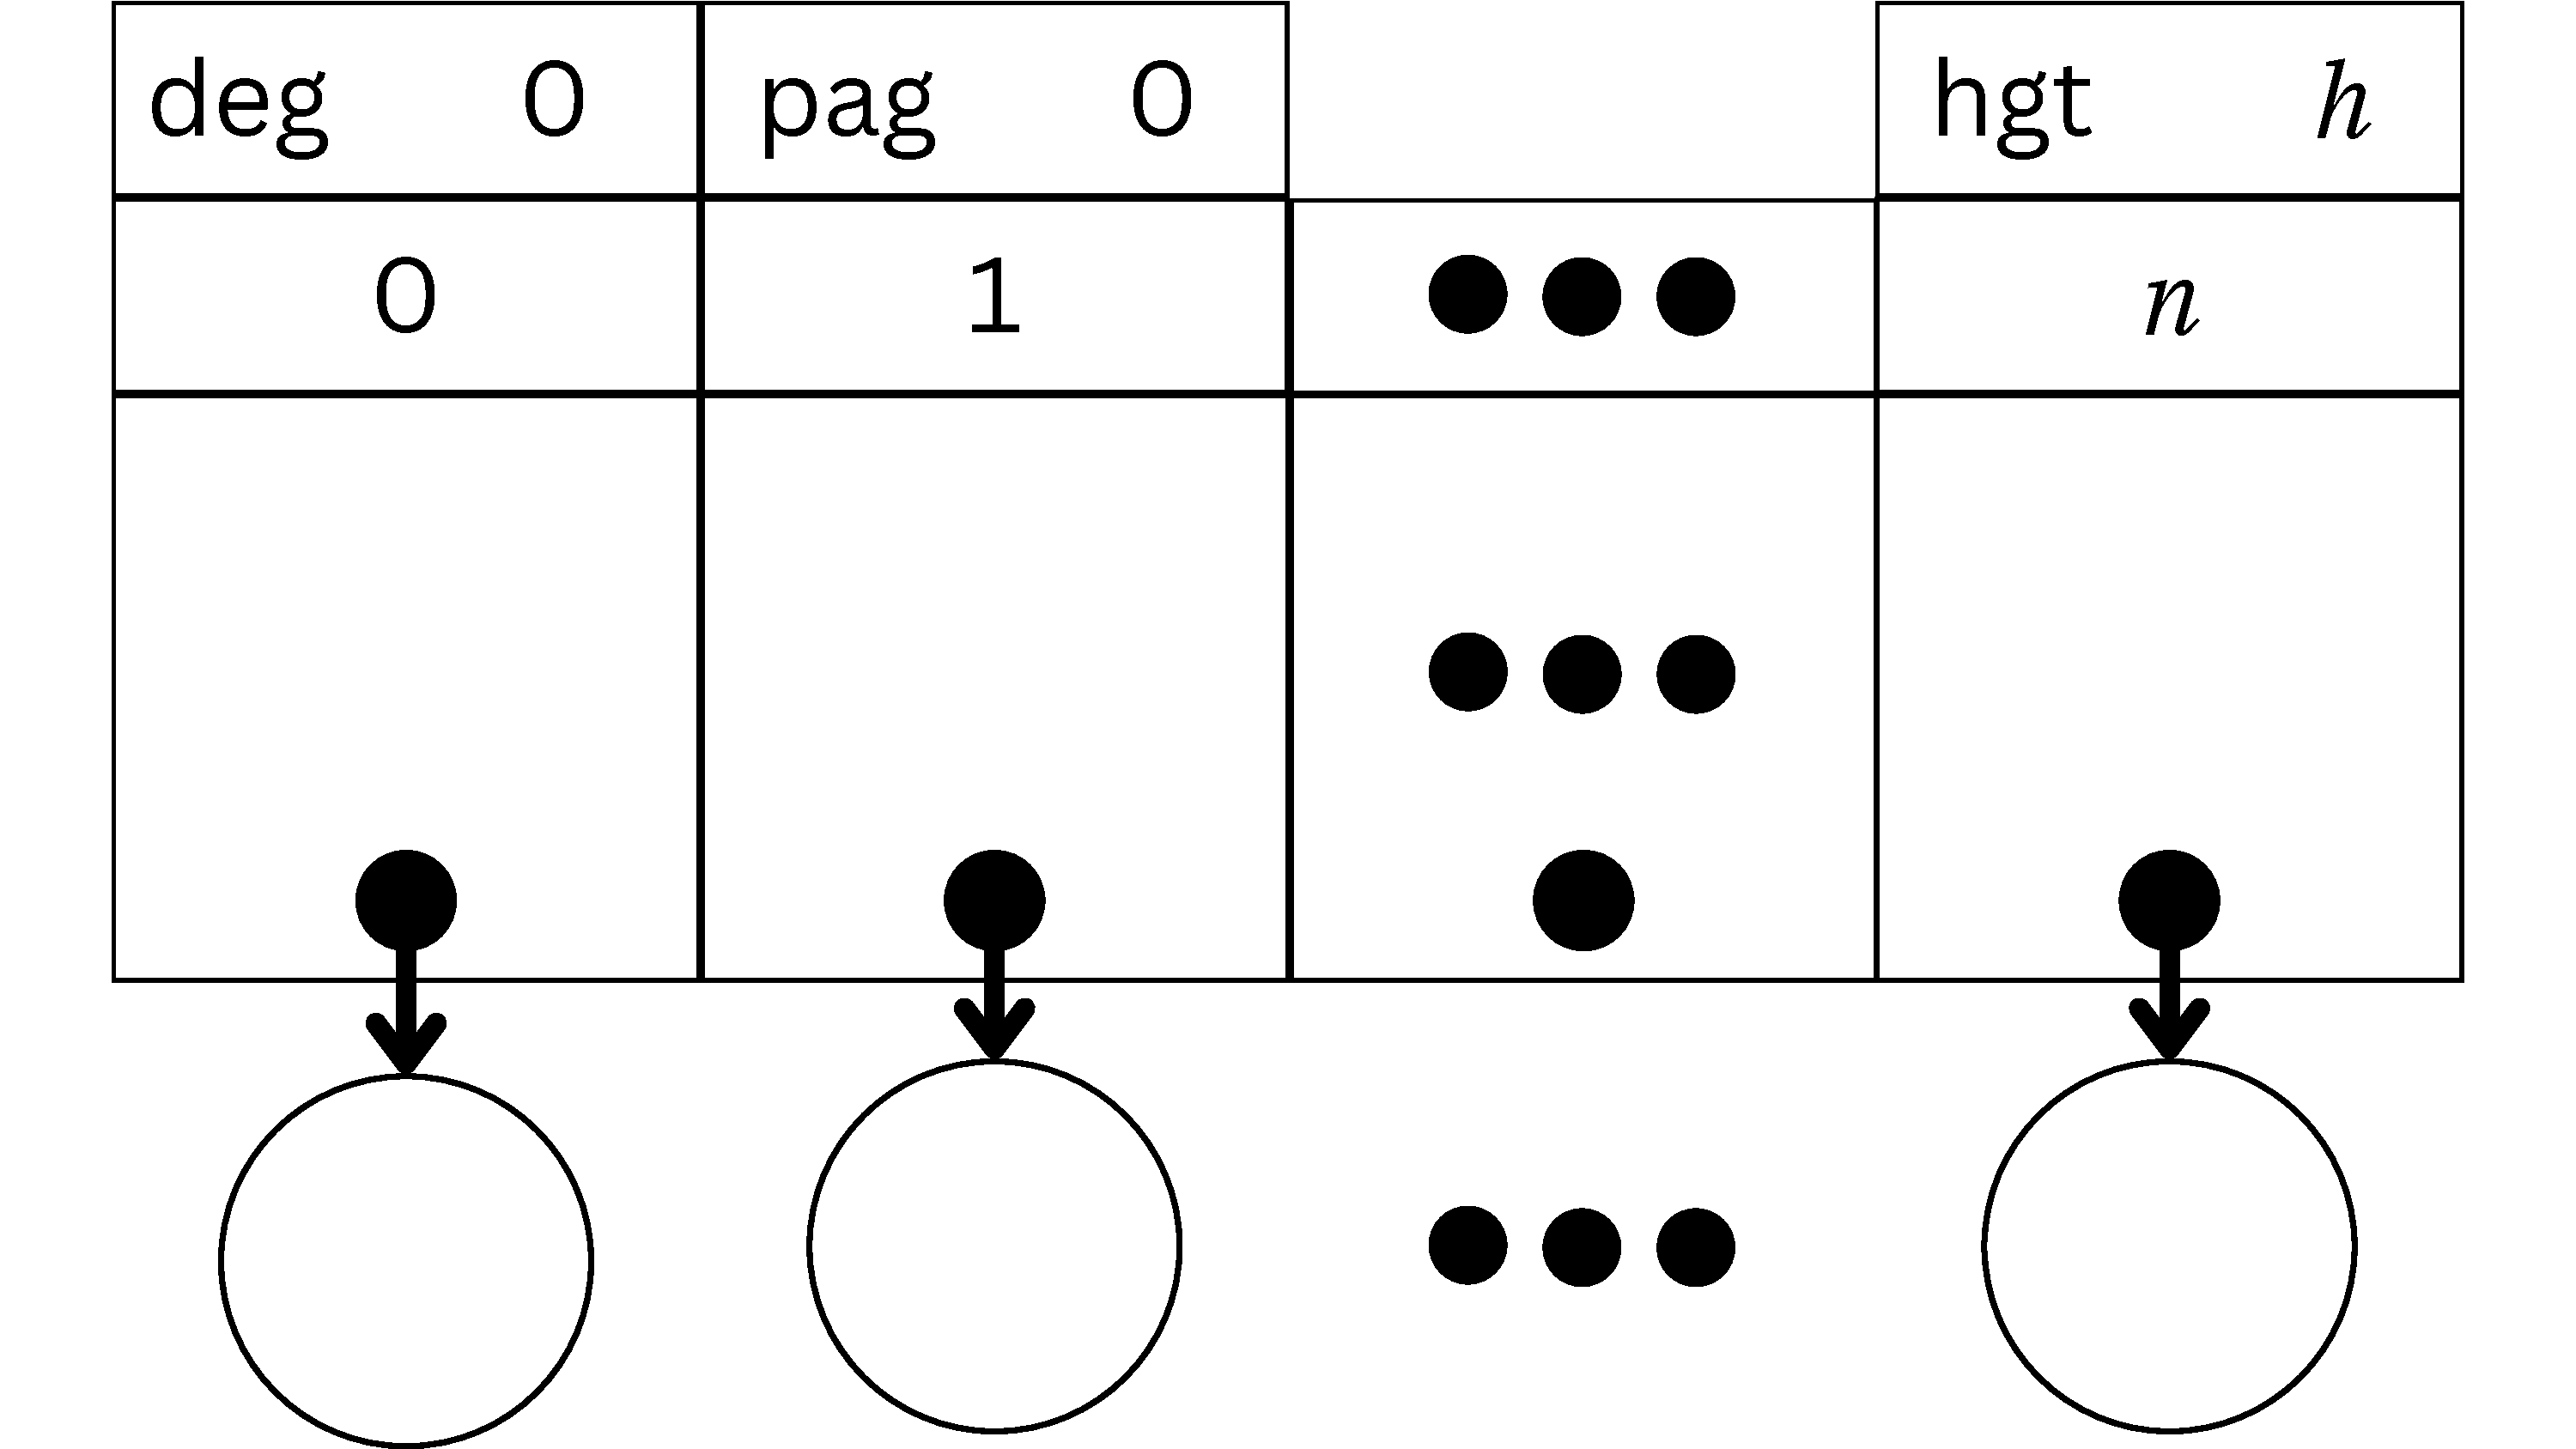
\includegraphics[%
                        width=\textwidth,%
                        page=1,%
                        ]{resources/made/B-Trees_general.pdf}
                    \caption[]{Leaf of a B-Tree}
                \end{figure}
        \end{column}
    \end{columns}
    \begin{figure}
        \includegraphics[%
            width=0.35\textwidth,%
            page=3,%
            ]{resources/made/B-Trees_general.pdf}
        \caption[]{Generic Node of a B-Tree}
    \end{figure}
\end{frame}


\begin{frame}[allowframebreaks]
    \subsection{Properties}
    \subsubsection{The \(\alpha\) Constant}
    \frametitle{B-Tree Properties---The \(\alpha\) constant}
    \begin{columns}
        \begin{column}{\textlecolumn}
            \begin{block}{}
                \begin{itemize}
                    \item The main property of the B-Trees is the \(\alpha\), a predefined constant.
                    \item The \(\alpha\) must be a Natural number, \(\alpha \in \mathbb{N}\) and \(\alpha \geq 2\).
                    \item This constant will determine the interval of keys and sub-trees, in a balanced node. This is called the \emph{Branching factor} of the tree.
                    \item The tree is balanced if they have from \(\alpha + 1\) to \(2\alpha + 1\) sub-trees in a single node.
                    \item Also, each balanced node have from \(\alpha\) to \(2\alpha\) keys.
                    \item The only node that can have less than \(\alpha + 1\) sub-trees and only 1 key is the \emph{Root} of the tree. 
                    \item But, the \emph{Root} still have the upper bounds of sub-trees and keys.
                \end{itemize}
            \end{block}
        \end{column}
        \begin{column}{\textricolumn}
        \end{column}
    \end{columns}
    \begin{columns}
        \begin{column}{0.5\textwidth}
                \begin{figure}
                    \includegraphics[%
                        width=0.45\textwidth,%
                        page=3,%
                        ]{resources/made/B-Trees_general.pdf}
                    \caption[]{Miminum Keys and Sub-Trees on a Node}
                \end{figure}
        \end{column}
        \begin{column}{0.5\textwidth}
                \begin{figure}
                    \includegraphics[%
                        width=0.45\textwidth,%
                        page=4,%
                        ]{resources/made/B-Trees_general.pdf}
                    \caption[]{Maximun Keys and Sub-Trees on a Node}
                \end{figure}
        \end{column}
    \end{columns}
    \framebreak{}
    \begin{columns}
        \begin{column}{\textlecolumn}
            \begin{block}{}
                \begin{figure}
                    \centering
                    \includegraphics[
                        width=0.9\linewidth,%
                        keepaspectratio,%
                        page=10,
                    ]{resources/made/B-Trees_general.pdf}
                    \caption[]{B-Tree, \(t\left(2,2\right)\)}
                \end{figure}
            \end{block}
        \end{column}
    \end{columns}
    \framebreak{}
    \begin{columns}
        \begin{column}{\textlecolumn}
            \begin{block}{}
                \vspace{-0.5cm}
                \begin{itemize}
                    \item We can prove the bounds of the number of sub-trees in a node, and define a function that let us get the number of sub-trees in a node.
                \end{itemize}
            \end{block}
        \end{column}
        \begin{column}{\textricolumn}
        \end{column}
    \end{columns}
    \begin{columns}
        \begin{column}{0.45\textwidth}
            \begin{block}{}
                \begin{proof}\renewcommand{\qedsymbol}{}
                    Let \(T \in t\left(\alpha, h\right)\), and \(N(T)\) be a function that returns the number of nodes in \(T\).
                    Let \(N_{\text{min}}\) and \(N_{\text{max}}\) the minimum and maximal number of nodes in \(T\). Then
                    \[
                        \begin{aligned}
                            N_{\text{min}} &= 1 + 2\left(\left(\alpha + 1\right){}^0 + \left(\alpha + 1\right){}^1 + \cdots + \left(\alpha + 1\right){}^{h-2} \right) \\
                            & = 1 + 2\left(\sum^{h - 2}_{i = 0} \left(\alpha + 1\right){}^i \right) \\
                            & = 1 + \frac{2}{\alpha}\left(\left(\alpha + 1\right){}^{h - 1} - 1\right)
                        \end{aligned}
                    \]
                \end{proof}
            \end{block}
        \end{column}
        \begin{column}{0.6\textwidth}
            \begin{figure}
                \includegraphics[%
                    width=\linewidth,%
                    keepaspectratio,%
                    page=5,%
                    ]{resources/made/B-Trees_general.pdf}
                \caption[]{B-Tree w/ the least number of nodes}
            \end{figure}
        \end{column}
    \end{columns}

    \framebreak{}

    \begin{columns}
        \begin{column}{0.4\textwidth}
            \begin{block}{}
                \begin{proof}[\unskip\nopunct]\renewcommand{\qedsymbol}{}
                    For \(h \geq 1\), we also have that
                    \[
                        \begin{aligned}
                            N_{\text{max}} &= 2\left(\sum^{h - 1}_{i = 0} \left(2\alpha + 1\right){}^i \right) \\
                            &= \frac{1}{2\alpha}\left(\left(2\alpha + 1\right){}^{h} - 1\right) \\
                        \end{aligned}
                    \]
                \end{proof}
            \end{block}
        \end{column}
        \begin{column}{0.6\textwidth}
            \begin{figure}
                \includegraphics[%
                    width=\linewidth,%
                    keepaspectratio,%
                    page=6,%
                    ]{resources/made/B-Trees_general.pdf}
                \caption[]{B-Tree w/ the most number of nodes}
            \end{figure}
        \end{column}
    \end{columns}
    \begin{columns}
        \begin{column}{\textlecolumn}
            \begin{block}{}
                \begin{proof}[\unskip\nopunct]
                    Then, if \(h = 0\), we have that \(N\left(T\right) = 0\). Else, if \(h \geq 1\)
                    \[
                        1 + \frac{2}{\alpha}\left(\left(\alpha + 1\right){}^{h - 1} - 1\right) 
                        \leq 
                        N\left(T\right) 
                        \leq 
                        \frac{1}{2\alpha}\left(\left(2\alpha + 1\right){}^{h} - 1\right)
                        \tag{Nodes Bounds}\label{btree-nodes-num}
                    \]
                \end{proof}
            \end{block}
        \end{column}
        \begin{column}{\textricolumn}
        \end{column}
    \end{columns}

    \framebreak{}

    \begin{columns}
        \begin{column}{\textlecolumn}
            \begin{block}{}
                \begin{itemize}
                    \item Keep in mind that the \emph{Branching Factor} of a B-Tree might change from each implementation, mostly in papers and books.
                    \item For example, on the original paper by Bayer and McCreight of B-Trees\cite{bayer_organization_1972}, the \emph{Branching Factor} 
                        goes from \(\alpha + 1\) to \(2\alpha + 1\) subtrees and from \(\alpha\) to \(2\alpha\) keys on a node.
                    \item But in the book made by Brass\cite{brass_advanced_2008}, the \emph{Branching Factor} goes from 
                        \(\alpha\) to \(2\alpha - 1\) for both, subtrees and keys in a node.
                    \item And on the original paper by Huddleston and Mehlhorn of AB-Trees\cite{huddleston_new_1982} keeps the same \emph{Branching Factor} as Brass.
                    \item But, we will see later that by limiting the upper bound of the \emph{Branching Factor} to something greater than \(2\alpha\) 
                        we will reach a even greater performance from this type of data structure.
                \end{itemize}
            \end{block}
        \end{column}
        \begin{column}{\textricolumn}
        \end{column}
    \end{columns}

\end{frame}

\begin{frame}[allowframebreaks,allowdisplaybreaks]
    \subsubsection{Keys and Sub-trees}
    \frametitle{B-Tree Properties---Keys and Sub-trees}
    \begin{columns}
        \begin{column}{\textlecolumn}
            \begin{block}{}
                \vspace{-0.8cm}
                \begin{itemize}
                    \item Each key has two sub-trees, one before and one after it. Like a normal tree.
                    \item First, let's define \(N\), a Node which isn't a leaf or \emph{Root}, from a B-Tree.
                    \item Then, we can define the set of the keys on a B-Tree Node \(N\) as \(\left\{k_1, k_2, \ldots{}, k_j\right\}\).
                    \item Leaving the index 0 for a placeholder, which is going to be used later.
                    \item Also, defining \(\symit{l}\) as the number of keys in \(N\).
                    \item Such that for \(t\left(\alpha, h\right)\), we have \(\alpha \leq \symit{l} \leq 2\alpha\).
                \end{itemize}
            \end{block}
        \end{column}
        \begin{column}{\textricolumn}
        \end{column}
    \end{columns}
    \begin{figure}[h!]
        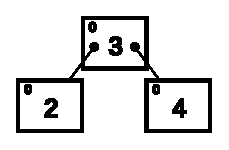
\includegraphics[height=0.175\linewidth]{resources/made/btree_2subtrees.eps}
        \caption{Simple node of a Normal Binary Tree}
    \end{figure}

    \framebreak

    \begin{columns}
        \begin{column}{\textlecolumn}
            \begin{block}{}
                \begin{itemize}
                    \item Now, we also define the set of sub-trees of \(N\) as \(\left\{p_0, p_1, \ldots{}, p_j\right\}\).
                    \item Where \(j\) is the number of sub-trees in \(N\).
                    \item Since there's a sub-tree before and after each key in \(N\).
                    \item Then, \(j\) must be equal to \(\symit{l} + 1\).
                    \item The keys and sub-trees are stored in a sequential increasing order.
                \end{itemize}
            \end{block}
        \end{column}
        \begin{column}{\textricolumn}
        \end{column}
    \end{columns}
    \begin{figure}[h!]
        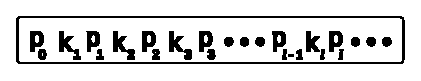
\includegraphics[width=0.85\linewidth]{resources/made/key_subtree_order.eps}
        \caption{Order of the Subtree Pointers and Keys.}
    \end{figure}

    \framebreak

    \begin{columns}
        \begin{column}{\textlecolumn}
            \begin{block}{}
                \begin{itemize}
                    \item In the case that \(N\) is the \emph{Root} of the tree, the only change is the minimum number of keys and sub-trees.
                    \item With \(\symit{l}\), already defined, \emph{Root} will have \(1 \leq \symit{l} \leq 2\alpha\) keys.
                    \item And \(2 \leq \symit{l} + 1 \leq 2\alpha + 1\) sub-trees.
                \end{itemize}
                \begin{itemize}
                    \item If \(N\) is a leaf of the tree, we are going to give the \(k_0\) a simple use.
                    \item The \(k_0\) will store a key value for an object.
                    \item This simple usage on a leaf is just one usage of the \(k_0\) on the nodes.
                \end{itemize}
            \end{block}
        \end{column}
        \begin{column}{\textricolumn}
            \begin{block}{}
            \end{block}
        \end{column}
    \end{columns}
    \begin{figure}
        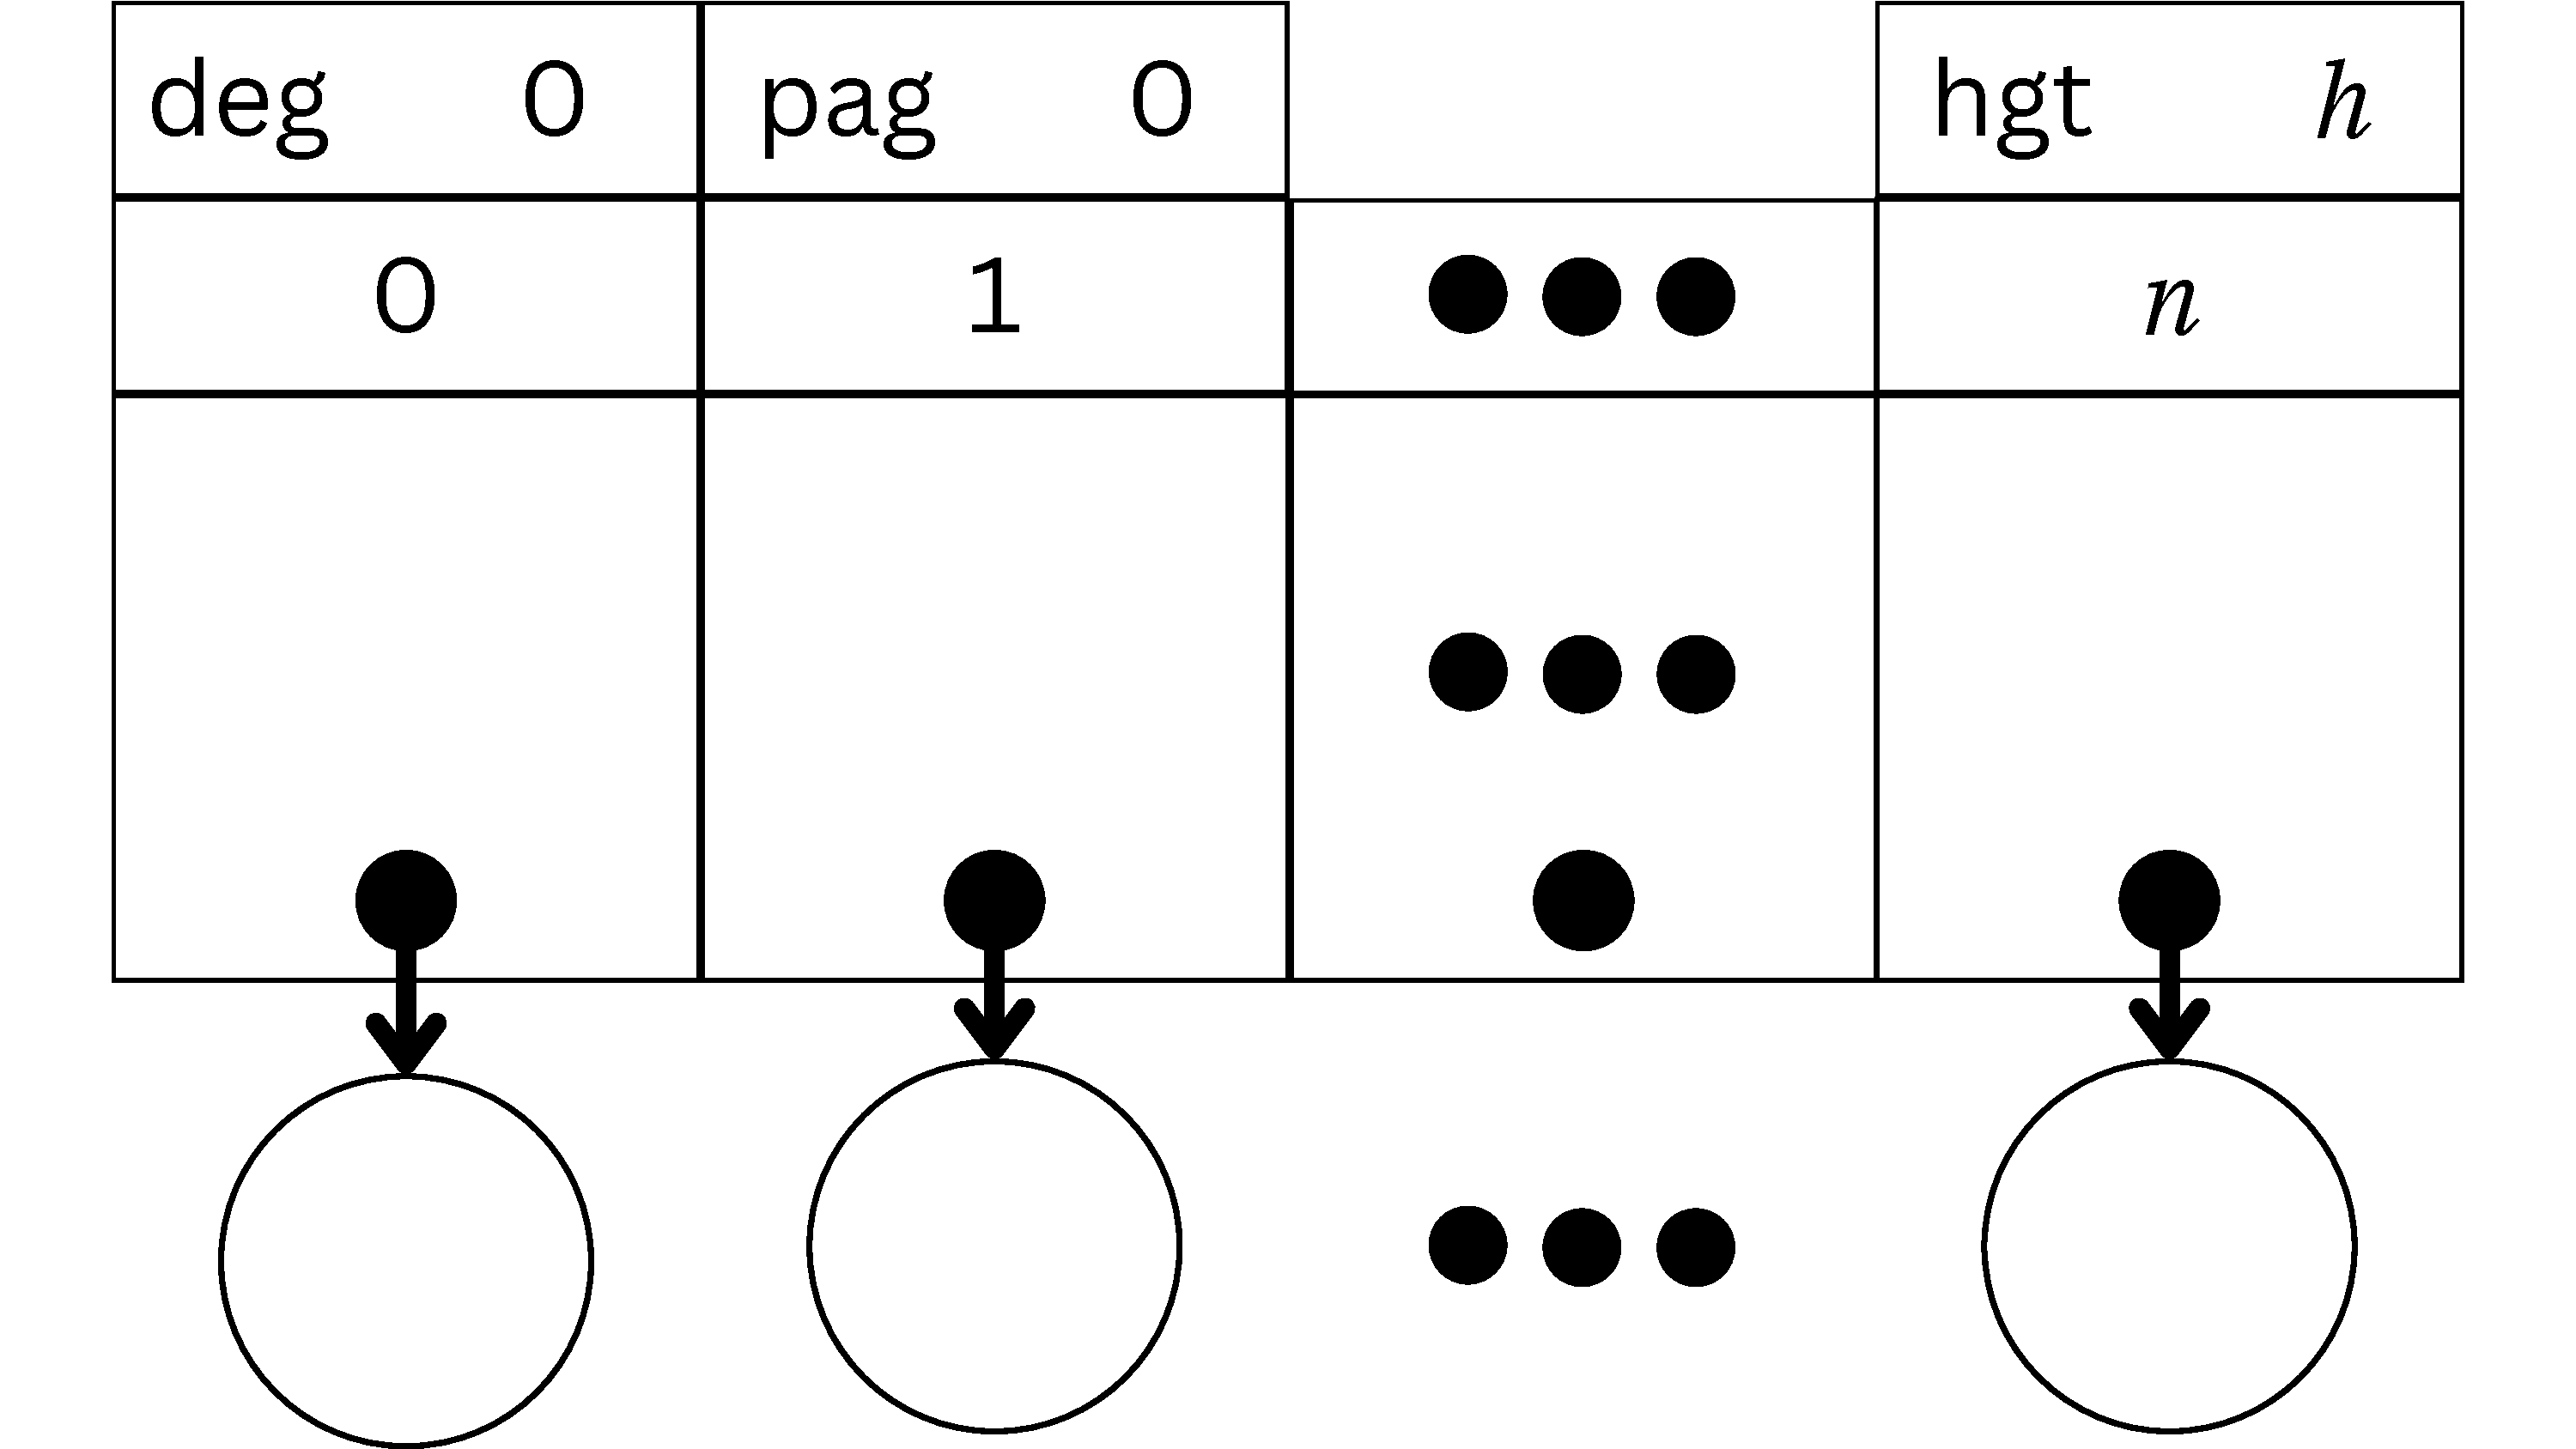
\includegraphics[%
            width=0.45\textwidth,%
            page=1,%
            ]{resources/made/B-Trees_general.pdf}
        \caption[]{Leaf of a B-Tree}
    \end{figure}
    \framebreak{}
    \begin{columns}
        \begin{column}{\textlecolumn}
            \begin{block}{}
                \begin{itemize}
                    \item Going back where \(N\) is a node on the B-Tree, but now this time \(N\) can be the tree \emph{Root}.
                    \item The order of the keys of \(p_i\), a subtree of \(N\); where \(0 \leq i \leq \symit{l}\), in comparison to the keys of \(N\) can be defined by 3 cases.
                    \item But first, we need to define \(K\left(T\right)\), where \(T \in t\left(\alpha, h\right)\), which is the set of keys inside the Node \(T\).
                    \item And, \(k_j \in K\left(N\right)\), where \(j\) is the index or position of the key in \(N\).
                \end{itemize}
                \vspace{0.5cm}
                \begin{align}
                    \forall y \in K\left(p_0\right);\mspace{20mu}& y < k_1 \tag{Case 1}\label{case1-subt-t-comp} \\
                    \forall y \in K\left(p_{i}\right);\mspace{20mu}& k_i \leq y < k_{i + 1};\mspace{20mu} 0 < i < \symit{l}, i \in \symbb{N} \tag{Case 2}\label{case2-subt-t-comp} \\
                    \forall y \in K\left(p_{\symit{l}}\right);\mspace{20mu}& k_{\symit{l}} \leq y \tag{Case 3}\label{case3-subt-t-comp}
                \end{align}
            \end{block}
        \end{column}
        \begin{column}{\textricolumn}
            \begin{block}{}
            \end{block}
        \end{column}
    \end{columns}
    \framebreak{}
    \begin{columns}
        \begin{column}{0.5\textwidth}
            \begin{figure}
                \centering{}
                \includegraphics[%
                    width=0.6\textwidth,%
                    page=7,%
                    ]{resources/made/B-Trees_general.pdf}
                \caption{Sub-tree Keys~\eqref{case1-subt-t-comp}}
            \end{figure}
        \end{column}
        \begin{column}{0.5\textwidth}
            \begin{figure}
                \centering{}
                \includegraphics[%
                    width=0.6\textwidth,%
                    page=8,%
                    ]{resources/made/B-Trees_general.pdf}
                \caption{Sub-tree Keys~\eqref{case3-subt-t-comp}}
            \end{figure}
        \end{column}
    \end{columns}
    \begin{figure}
        \centering{}
        \includegraphics[%
            width=0.45\textwidth,%
            page=9,%
            ]{resources/made/B-Trees_general.pdf}
        \caption{Sub-tree Keys~\eqref{case2-subt-t-comp}}
    \end{figure}
\end{frame}

\begin{frame}[allowframebreaks,allowdisplaybreaks]
    \subsubsection{Height}
    \frametitle{B-Tree Properties---Height}
    \begin{columns}
        \begin{column}{\textlecolumn}
            \begin{block}{}
                \begin{itemize}
                    \item Before we can define and prove the height of a B-Tree we need to define some things.
                    \item First, The set of the keys in \(T \in t\left(\alpha, h\right)\) will be defined as \(I\). 
                    \item Now, The \(I_{\text{min}}\) and \(I_{\text{max}}\) of \(T\) can be easily defined by \eqref{btree-nodes-num}:
                \end{itemize}
            \end{block}
            \vspace{-0.35cm}
            \begin{tcolorbox}[boxsep=0mm,left=0mm,right=0mm,top=-2mm,halign=right]
                \[
                    1 + 2\frac{\left(\left(\alpha + 1\right)^{h - 1} - 1\right)}{\alpha} 
                    \leq 
                    N\left(T\right) 
                    \leq 
                    \frac{\left(\left(2\alpha + 1\right)^{h} - 1\right)}{2\alpha}
                \]
            \end{tcolorbox}
        \end{column}
        \begin{column}{\textricolumn}
        \end{column}
    \end{columns}
    \begin{columns}
        \begin{column}{0.5\textwidth}
            \vspace{-0.75cm}
            \begin{block}{}
                \[
                    \begin{aligned}
                        I_{\text{min}} &= 1 + \alpha\left(N_{\text{min}}\left(T\right) - 1\right) \\
                        &= 1 + \alpha\left(\frac{2\left(\alpha + 1\right)^{h - 1} - 2}{\alpha}\right) \\
                        &= 2\left(\alpha + 1\right)^{h - 1} - 1
                    \end{aligned}
                \]
            \end{block}
        \end{column}
        \begin{column}{0.5\textwidth}
            \begin{figure}
                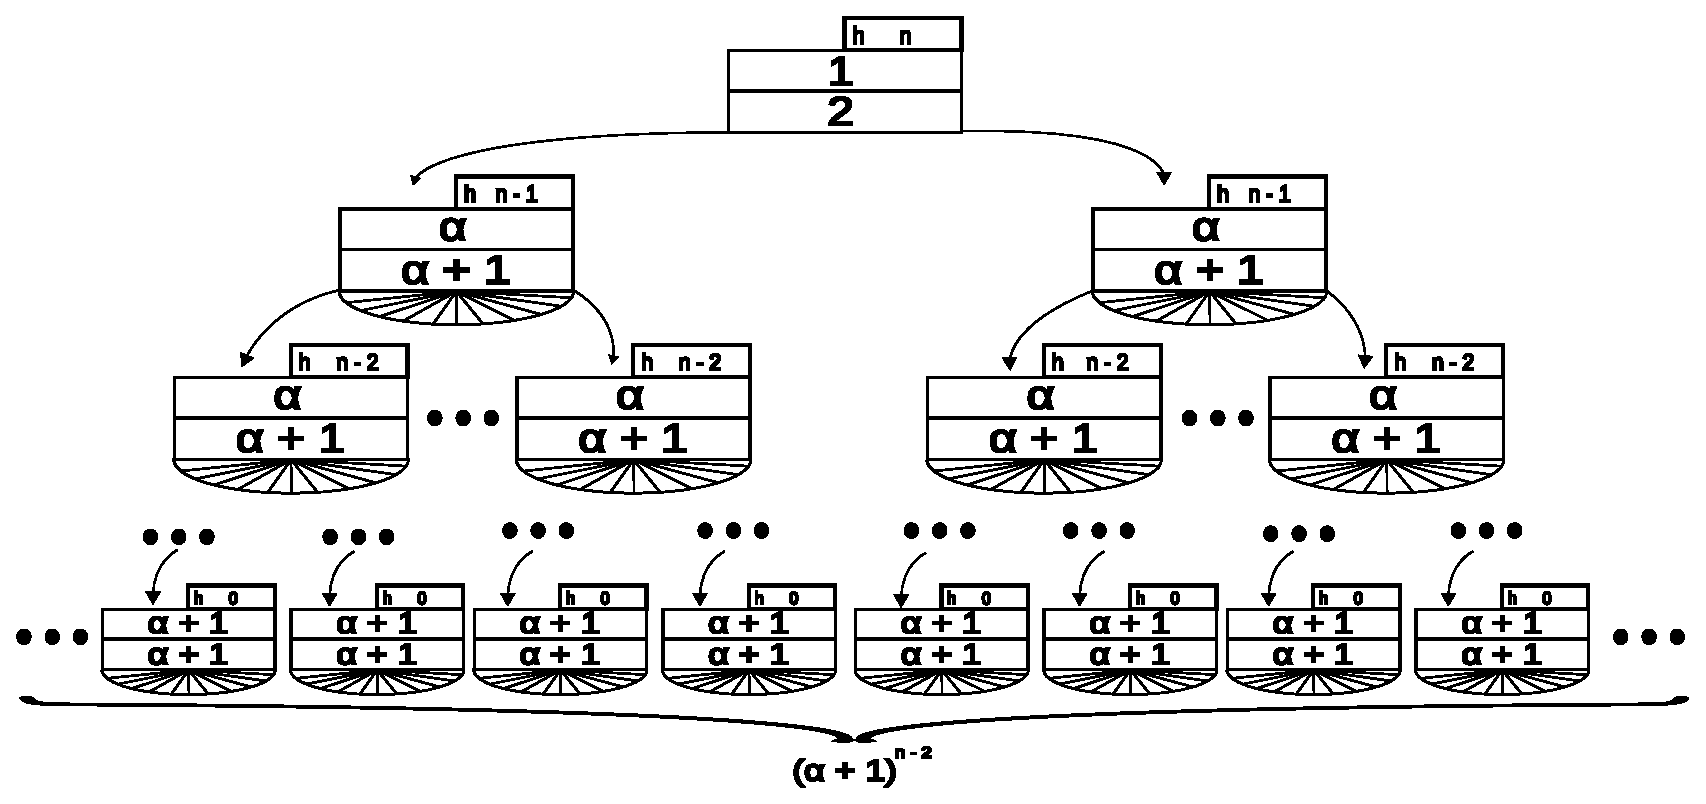
\includegraphics[width=0.95\linewidth,keepaspectratio]{resources/made/generic_min_btree.eps}
                \caption[]{B-Tree w/ the least number of nodes}
            \end{figure}
        \end{column}
    \end{columns}

    \framebreak

    \begin{columns}
        \begin{column}{0.5\textwidth}
            \begin{block}{}
                \vspace{-0.75cm}
                \[
                    \begin{aligned}
                        I_{\text{max}} &= 2\alpha\left(N_{\text{max}}\left(T\right)\right) \\
                        &= 2\alpha \left(\frac{\left(2\alpha + 1\right)^h - 1}{2\alpha}\right) \\
                        &= \left(2\alpha + 1\right)^h - 1
                    \end{aligned}
                \]
            \end{block}
        \end{column}
        \begin{column}{0.5\textwidth}
            \begin{figure}
                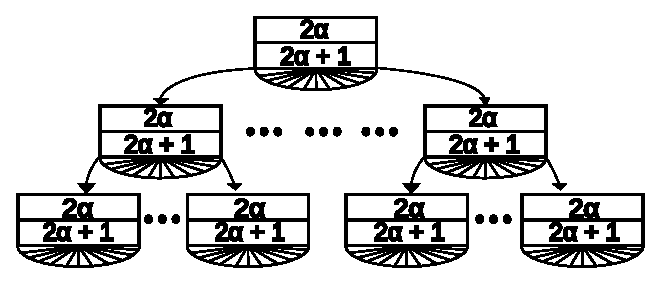
\includegraphics[width=0.95\linewidth,keepaspectratio]{resources/made/generic_max_btree.eps}
                \caption[]{B-Tree w/ the most number of nodes}
            \end{figure}
        \end{column}
    \end{columns}
    \begin{itemize}
        \item Now, we can solve for \(h\) with each bound of \(I\) and define an bound of h with them.
    \end{itemize}
    \begin{columns}
        \begin{column}{0.5\textwidth}
            \begin{block}{}
                \[
                    \begin{aligned}
                        I_{\text{min}} &= 2\left(\alpha + 1\right)^{h - 1} - 1 \\
                        \frac{I_{\text{min} + 1}}{2} &= \left(\alpha + 1\right)^{h - 1} \\
                        \log_{\alpha + 1}\left(\frac{I_{\text{min}} + 1}{2} + 1\right) &= h_{\text{min}}
                    \end{aligned}
                \]
            \end{block}
        \end{column}
        \begin{column}{0.5\textwidth}
            \[
                \begin{aligned}
                    I_{\text{max}} &= \left(2\alpha + 1\right)^h - 1 \\
                    I_{\text{max}} + 1 &= \left(2\alpha + 1\right)^h \\
                    \log_{2\alpha + 1} \left(I_{\text{max}} + 1\right) = h_{\text{max}}
                \end{aligned}
            \]
        \end{column}
    \end{columns}

    \framebreak

    \begin{columns}
        \begin{column}{\textlecolumn}
            \begin{block}{}
                \begin{itemize}
                    \item Since, \(2\alpha + 1 > \alpha + 1\), then \(log_{2\alpha + 1} x \leq log_{\alpha + 1}x\), both in \(\left[1, \infty\right)\).
                    \item Or also, if we have more nodes in a B-Tree, the height of the Tree will be less than if we have less nodes in the B-Tree.
                    \item Hence, for \(I \geq 1\), we will have the bounds for \(h\):
                \end{itemize}
                \[
                    \log_{2\alpha + 1}\left(I + 1\right)
                    \leq
                    h
                    \leq
                    \log_{\alpha + 1}\left(\frac{I + 1}{2} + 1\right)
                \]
                \begin{itemize}
                    \item And if, \(I = 0\) then, \(h = 0\).
                \end{itemize}
            \end{block}
        \end{column}
        \begin{column}{\textricolumn}
        \end{column}
    \end{columns}
\end{frame}

\begin{frame}
    \frametitle{B-Tree Properties---Summary}
    \begin{columns}
        \begin{column}{\textlecolumn}
            \begin{block}{}
                \begin{itemize}
                    \item A B-Tree is defined as: \(T \in t\left(\alpha, h\right)\)
                    \item A B-Tree has a predefined constant \(\alpha\).
                    \item Node can have \(\alpha \leq I \leq 2\alpha\) keys.
                    \item Also, it has \(\alpha + 1 \leq I + 1 \leq 2\alpha + 1\) sub-trees.
                    \item Except the \emph{Root} node, which can have at least 1 key and 2 sub-trees.
                    \item The leafs use the \(k_0\) space to store object key information.
                    \item For each key on sub-tree of a Node, there's 3 cases:
                        \begin{align*}
                            \forall y \in K\left(p_0\right);\mspace{20mu}& y < k_1 \\
                            \forall y \in K\left(p_{i}\right);\mspace{20mu}& k_i \leq y < k_{i + 1};\mspace{20mu} 0 < i < \symit{l} \wedge i \in \symbb{N} \\
                            \forall y \in K\left(p_{\symit{l}}\right);\mspace{20mu}& k_{\symit{l}} \leq y
                        \end{align*}
                    \item The number of nodes of a B-Tree is bounded by:
                        \(
                            1 + \frac{2}{\alpha}\left(\left(\alpha + 1\right){}^{h - 1} - 1\right) 
                            \leq 
                            N\left(T\right) 
                            \leq 
                            \frac{1}{2\alpha}\left(\left(2\alpha + 1\right){}^{h} - 1\right)
                        \)
                    \item The number of Keys in a B-Tree is bounded by:
                        \(
                            2\left(\alpha + 1\right){}^{h - 1} - 1 
                            \leq 
                            I 
                            \leq
                            \left(2\alpha + 1\right){}^h - 1
                        \)
                    \item The height of a B-Tree is bounded by:
                        \[
                            \log_{2\alpha + 1}\left(I + 1\right)
                            \leq
                            h
                            \leq
                            \log_{\alpha + 1}\left(\frac{I + 1}{2} + 1\right)
                        \]
                \end{itemize}
            \end{block}
        \end{column}
        \begin{column}{\textricolumn}
        \end{column}
    \end{columns}
\end{frame}



\begin{frame}
    \subsection{Structure}
    \frametitle{B-Tree Structure}
    \begin{columns}
        \begin{column}{\textlecolumn}
            \begin{block}{}
                \begin{itemize}
                    \item The structure of the B-Tree's node adds two arrays where the keys and sub-trees' pointers will be stored:
                \end{itemize}
                \inputminted[%
                    linenos,%
                    breakbytoken,%
                    highlightlines={1,2,6,7}%
                    ]{c}{resources/code/b_tree_struct.c}
            \end{block}
        \end{column}
        \begin{column}{\textricolumn}
        \end{column}
    \end{columns}
\end{frame}


\begin{frame}
    \subsection{Operations}
    \frametitle{B-Tree Operations}
    \begin{columns}
        \begin{column}{\textlecolumn}
            \begin{block}{}
                \begin{itemize}
                    \item For these operations, we will assume that the whole B-Tree is loaded into main memory.
                    \item We have to asume this since the main usage of the B-Tree is oriented to secondary storage.
                    \item Generally, only the \emph{Root} and node to operate, if available, will be always available in memory.
                    \item But if we need any other node, we will have to read into our secondary memory and fetch it's data.
                    \item This process takes more time than the general data fetch from main memory.
                    \item So, the fewer times we do this process the better.
                \end{itemize}
            \end{block}
        \end{column}
        \begin{column}{\textricolumn}
        \end{column}
    \end{columns}
    \begin{figure}[h!]
        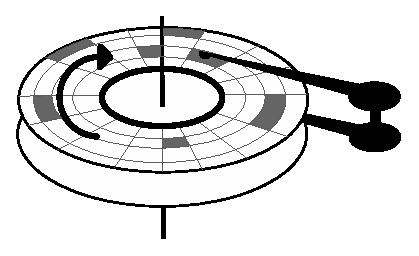
\includegraphics[width=0.5\textwidth]{resources/made/external_storage_wblocks.eps}
        \caption{External storage with the sectors to access highlighted}
    \end{figure}
\end{frame}


\begin{frame}
    \subsubsection{Creating an empty B-Tree}
    \frametitle{B-Tree Operations---Creating an empty B-Tree}
    \begin{columns}
        \begin{column}{\textlecolumn}
            \begin{block}{}
                \begin{itemize}
                    \item We use \lstinline|create_tree()| to create a empty B-Tree, and since we only need to use \lstinline|get_node()|, this operation takes \(\Theta(1)\).
                \end{itemize}
            \end{block}
        \end{column}
        \begin{column}{\textricolumn}
        \end{column}
    \end{columns}
    \inputminted[%
        linenos,%
        breakbytoken,%
        highlightlines={3,6}%
        ]{c}{resources/code/b_tree_create.c}
\end{frame}


\begin{frame}[t,allowframebreaks,allowdisplaybreaks]
    \subsubsection{Search value}
    \frametitle{B-Tree Operations---Search}
    \vspace{-1cm}
    \begin{columns}
        \begin{column}{\textlecolumn}
            \begin{block}{}
                \begin{itemize}
                    \item The changes of this operations are mainly focused on the search part, since we have to compare to an array of keys and not only the node key.
                    \item This operation returns the object in the B-Tree if a given key exists.
                \end{itemize}
            \end{block}
        \end{column}
        \begin{column}{\textricolumn}
        \end{column}
    \end{columns}
    \inputminted[
        highlightlines={6,12,19,22,27}
    ]{c}{resources/code/b_tree_find.c}
    \begin{figure}[h!]
        \includegraphics[%
            width=0.55\linewidth,%
            page=62%
        ]{resources/made/B-Trees_insert_example.pdf}
    \end{figure}
    \begin{itemize}
        \item Let's search for \(70\) in this \(t\left(2,2\right)\) B-Tree.
    \end{itemize}
\end{frame}

\begin{frame}[t,allowframebreaks,allowdisplaybreaks]
    \frametitle{B-Tree Operations---Search (Example)}
\end{frame}


\begin{frame}[t,allowframebreaks, allowdisplaybreaks]
    \subsubsection{Insert}
    \frametitle{B-Tree Operations---Insert Value}
    \begin{columns}
        \begin{column}{\textlecolumn}
            \begin{block}{}
                \begin{itemize}
                    \item The insertion algorithm in the B-Tree almost has nothing to share with any tree insertion algorithm.
                    \item The first section of the code is the same \lstinline|find| algorithm so we can see if the value to add is already 
                        stored in the B-Tree and where could it be stored, also storing in a stack the nodes that we are going to access.
                    \item Then, if the node isn't full yet, we are just going to move everything by an index until the current elements are 
                        less than the key that we are going to insert.
                    \item But, if the node is full, we will get a new node for the B-Tree and split in half the full node.
                    \item Then, insert the new key into one of thoose of the splited nodes.
                    \item Then, the median key of the splited node will be taken from the nodes and will be inserted on the upper node.
                    \item In the new insertion of the median key and new node, will be repeated until we have a non-full node which can 
                        take another element, or if we reach the root node we will have to do a extra process.
                    \item This extra process is that we have to split the root node, create a new node and increase the height of the B-Tree by inserting the new node with 
                        keys, pointers and such to the rest of the B-Tree above everything.
                    \item \textbf{This is one of the only ways that the B-Tree can change it's height.}
                \end{itemize}
            \end{block}
        \end{column}
        \begin{column}{\textricolumn}
        \end{column}
    \end{columns}
    
    \framebreak{}

    \inputminted[
        highlightlines={13, 14, 17, 20, 26, 30, 31, 33, 35, 38, 42, 45, 56, 64, 65, 66, 67, 81, 98, 99, 100, 102, 103, 104, 108, 110, 111, 117, 119, 121, 122, 123, 124, 125, 126, 130, 131},
    ]{c}{resources/code/b_tree_insert.c}

    \begin{figure}[h!]
        \includegraphics[%
            width=0.45\linewidth,%
            page=1%
        ]{resources/made/B-Trees_insert_example.pdf}
    \end{figure}

    \begin{itemize}
        \item Now, lets create a new empty tree and insert a lot of elements in a \(t\left(2, 0\right)\) B-Tree. With the bounds \(\alpha\) and \(2\alpha - 1\).
    \end{itemize}
\end{frame}

\begin{frame}[allowframebreaks, allowdisplaybreaks]
    \frametitle{B-Tree Operations---Insert (Example)}
    \newcounter{insert-example}
    \newcounter{insert-img-example}
    \newcounter{insert-step-example}[insert-example]
    \setcounter{insert-example}{0}
    \setcounter{insert-img-example}{0}
    \setcounter{insert-step-example}{0}
    % insert 1
    \stepcounter{insert-example}
    \stepcounter{insert-img-example}
	\stepcounter{insert-step-example}
    \begin{columns}
        \begin{column}{.47\textwidth}
            \inputminted[%
                highlightlines={1,2,3,4,5},%
                firstline=1,%
                lastline=11,%
                tabsize=1,%
                fontsize=\examplefnt,%
            ]{c}{resources/code/b_tree_insert.c}
        \end{column}
        \begin{column}{.5\textwidth}
            \examplefnt{%
                \begin{itemize}
                    \item Insert \arabic{insert-example}; Step \arabic{insert-step-example};
                    \item \hlght{tree=(*pag 0); new\_key=50; new\_object=(*50);}
                    \item finished; insert\_key;
                    \item \hlght{current\_node=(*pag 0);}
                \end{itemize}
            }
        \end{column}
    \end{columns}
    \begin{figure}[h!]
        \includegraphics[%
            width=0.45\linewidth,%
            page=\value{insert-img-example}%
        ]{resources/made/B-Trees_insert_example.pdf}
    \end{figure}
    \framebreak{}
    \stepcounter{insert-img-example}
	\stepcounter{insert-step-example}
    \stepcounter{insert-img-example}
    \begin{columns}
        \begin{column}{.47\textwidth}
            \inputminted[%
                highlightlines={6,7,8,9,10},%
                firstline=1,%
                lastline=11,%
                tabsize=1,%
                fontsize=\examplefnt,%
            ]{c}{resources/code/b_tree_insert.c}
        \end{column}
        \begin{column}{.5\textwidth}
            \examplefnt{%
                \begin{itemize}
                    \item Insert \arabic{insert-example}; Step \arabic{insert-step-example};
                    \item tree=(*pag 0); 
                        new\_key=50; 
                        new\_object=(*50);
                    \item finished; insert\_key;
                    \item current\_node=(*pag 0);
                \end{itemize}
            }
        \end{column}
    \end{columns}
    \begin{figure}[h!]
        \includegraphics[%
            width=0.45\linewidth,%
            page=\value{insert-img-example}%
        ]{resources/made/B-Trees_insert_example.pdf}
    \end{figure}
    \framebreak{}
    % Insert 2
    \stepcounter{insert-example}
    \stepcounter{insert-img-example}
	\stepcounter{insert-step-example}
    \begin{columns}
        \begin{column}{.47\textwidth}
            \inputminted[%
                highlightlines={6},%
                firstline=6,%
                lastline=6,%
                tabsize=1,%
                fontsize=\examplefnt,%
            ]{c}{resources/code/b_tree_insert.c}
            \inputminted[%
                highlightlines={13, 14},%
                firstline=13,%
                lastline=27,%
                tabsize=1,%
                fontsize=\examplefnt,%
            ]{c}{resources/code/b_tree_insert.c}
        \end{column}
        \begin{column}{.5\textwidth}
            \examplefnt{%
                \begin{itemize}
                    \item Insert \arabic{insert-example}; Step \arabic{insert-step-example};
                    \item \hlght{tree=(*pag 0); new\_key=20; new\_object=(*20);}
                    \item finished; insert\_key;
                    \item \hlght{current\_node=(*pag 0);}
                \end{itemize}
            }
        \end{column}
    \end{columns}
    \begin{figure}[h!]
        \includegraphics[%
            width=0.45\linewidth,%
            page=\value{insert-img-example}%
        ]{resources/made/B-Trees_insert_example.pdf}
    \end{figure}
    \framebreak{}
    \stepcounter{insert-img-example}
	\stepcounter{insert-step-example}
    \begin{columns}
        \begin{column}{.47\textwidth}
            \inputminted[%
                highlightlines={32,33,34,35,38,39},%
                firstline=30,%
                lastline=40,%
                tabsize=1,%
                fontsize=\examplefnt,%
            ]{c}{resources/code/b_tree_insert.c}
        \end{column}
        \begin{column}{.5\textwidth}
            \examplefnt{%
                \begin{itemize}
                    \item Insert \arabic{insert-example}; Step \arabic{insert-step-example};
                    \item tree=(*pag 0); new\_key=20; new\_object=(*20);
                    \item \hlght{finished=0; insert\_key=20; insert\_pt=(*20);}
                    \item current\_node=(*pag 0);
                    \item \hlght{i; start=0;}
                \end{itemize}
            }
        \end{column}
    \end{columns}
    \begin{figure}[h!]
        \includegraphics[%
            width=0.45\linewidth,%
            page=\value{insert-img-example},%
        ]{resources/made/B-Trees_insert_example.pdf}
    \end{figure}
    \framebreak{}
    \stepcounter{insert-img-example}
	\stepcounter{insert-step-example}
    \begin{columns}
        \begin{column}{.47\textwidth}
            \inputminted[%
                highlightlines={42,44,45,46,47},%
                firstline=41,%
                lastline=49,%
                tabsize=1,%
                fontsize=\examplefnt,%
            ]{c}{resources/code/b_tree_insert.c}
        \end{column}
        \begin{column}{.5\textwidth}
            \examplefnt{%
                \begin{itemize}
                    \item Insert \arabic{insert-example}; Step \arabic{insert-step-example};
                    \item tree=(*pag 0); new\_key=20; new\_object=(*20);
                    \item finished=0; insert\_key=20; insert\_pt=(*20);
                    \item current\_node=(*pag 0);
                    \item \hlght{i=1 \rarr{} 0}; start=0;
                \end{itemize}
            }
        \end{column}
    \end{columns}
    \begin{figure}[h!]
        \includegraphics[%
            width=0.45\linewidth,%
            page=\value{insert-img-example},%
        ]{resources/made/B-Trees_insert_example.pdf}
    \end{figure}
    \framebreak{}
    \stepcounter{insert-img-example}
	\stepcounter{insert-step-example}
    \begin{columns}
        \begin{column}{.47\textwidth}
            \inputminted[%
                highlightlines={51,52,53,54},%
                firstline=51,%
                lastline=55,%
                tabsize=1,%
                fontsize=\examplefnt,%
            ]{c}{resources/code/b_tree_insert.c}
            \inputminted[%
                highlightlines={125,126},%
                firstline=125,%
                lastline=127,%
                tabsize=1,%
                fontsize=\examplefnt,%
            ]{c}{resources/code/b_tree_insert.c}
        \end{column}
        \begin{column}{.5\textwidth}
            \examplefnt{%
                \begin{itemize}
                    \item Insert \arabic{insert-example}; Step \arabic{insert-step-example};
                    \item tree=(*pag 0); new\_key=20; new\_object=(*20);
                    \item \hlght{finished=1}; insert\_key=20; insert\_pt=(*20);
                    \item current\_node=(*pag 0);
                    \item i=0; start=0;
                \end{itemize}
            }
        \end{column}
    \end{columns}
    \includegraphics[%
        width=0.45\linewidth,%
        page=\value{insert-img-example},%
    ]{resources/made/B-Trees_insert_example.pdf}
    \framebreak{}
    % Insert 3 
    \stepcounter{insert-example}
    \stepcounter{insert-img-example}
	\stepcounter{insert-step-example}
    \begin{columns}
        \begin{column}{.47\textwidth}
            \inputminted[%
                highlightlines={},%
                firstline=6,%
                lastline=6,%
                tabsize=1,%
                fontsize=\examplefnt,%
            ]{c}{resources/code/b_tree_insert.c}
            \inputminted[%
                highlightlines={},%
                firstline=13,%
                lastline=14,%
                tabsize=1,%
                fontsize=\examplefnt,%
            ]{c}{resources/code/b_tree_insert.c}
            \inputminted[%
                highlightlines={39},%
                firstline=30,%
                lastline=40,%
                tabsize=1,%
                fontsize=\examplefnt,%
            ]{c}{resources/code/b_tree_insert.c}
        \end{column}
        \begin{column}{.5\textwidth}
            \examplefnt{%
                \begin{itemize}
                    \item Insert \arabic{insert-example}; Step \arabic{insert-step-example};
                    \item tree=(*pag 0); \hlght{new\_key=70; new\_object=(*70);}
                    \item finished=0; \hlght{insert\_key=70; insert\_pt=(*70);}
                    \item current\_node=(*pag 0);
                    \item i; start=0;
                \end{itemize}
            }
        \end{column}
    \end{columns}
    \includegraphics[%
        width=0.45\linewidth,%
        page=\value{insert-img-example},%
    ]{resources/made/B-Trees_insert_example.pdf}
    \framebreak{}
    \stepcounter{insert-img-example}
	\stepcounter{insert-step-example}
    \begin{columns}
        \begin{column}{.47\textwidth}
            \inputminted[%
                highlightlines={42,45},%
                firstline=41,%
                lastline=49,%
                tabsize=1,%
                fontsize=\examplefnt,%
            ]{c}{resources/code/b_tree_insert.c}
        \end{column}
        \begin{column}{.5\textwidth}
            \examplefnt{%
                \begin{itemize}
                    \item Insert \arabic{insert-example}; Step \arabic{insert-step-example};
                    \item tree=(*pag 0); new\_key=70; new\_object=(*70);
                    \item finished=0; insert\_key=70; insert\_pt=(*70);
                    \item current\_node=(*pag 0);
                    \item \hlght{i=2; start=0};
                \end{itemize}
            }
        \end{column}
    \end{columns}
    \includegraphics[%
        width=0.45\linewidth,%
        page=\value{insert-img-example},%
    ]{resources/made/B-Trees_insert_example.pdf}
    \framebreak{}
    \stepcounter{insert-img-example}
	\stepcounter{insert-step-example}
    \begin{columns}
        \begin{column}{.47\textwidth}
            \inputminted[%
                highlightlines={54},%
                firstline=51,%
                lastline=55,%
                tabsize=1,%
                fontsize=\examplefnt,%
            ]{c}{resources/code/b_tree_insert.c}
            \inputminted[%
                highlightlines={126},%
                firstline=125,%
                lastline=127,%
                tabsize=1,%
                fontsize=\examplefnt,%
            ]{c}{resources/code/b_tree_insert.c}
        \end{column}
        \begin{column}{.5\textwidth}
            \examplefnt{%
                \begin{itemize}
                    \item Insert \arabic{insert-example}; Step \arabic{insert-step-example};
                    \item tree=(*pag 0); new\_key=70; new\_object=(*70);
                    \item \hlght{finished=1}; insert\_key=70; insert\_pt=(*70);
                    \item current\_node=(*pag 0);
                    \item i=2; start=0;
                \end{itemize}
            }
        \end{column}
    \end{columns}
    % Insert 4 
    \includegraphics[%
        width=0.45\linewidth,%
        page=\value{insert-img-example},%
    ]{resources/made/B-Trees_insert_example.pdf}
    \stepcounter{insert-example}
    \framebreak{}
    \stepcounter{insert-img-example}
	\stepcounter{insert-step-example}
    \begin{columns}
        \begin{column}{.47\textwidth}
            \inputminted[%
                highlightlines={6},%
                firstline=6,%
                lastline=6,%
                tabsize=1,%
                fontsize=\examplefnt,%
            ]{c}{resources/code/b_tree_insert.c}
            \inputminted[%
                highlightlines={14},%
                firstline=13,%
                lastline=14,%
                tabsize=1,%
                fontsize=\examplefnt,%
            ]{c}{resources/code/b_tree_insert.c}
            \inputminted[%
                highlightlines={39},%
                firstline=30,%
                lastline=40,%
                tabsize=1,%
                fontsize=\examplefnt,%
            ]{c}{resources/code/b_tree_insert.c}
        \end{column}
        \begin{column}{.5\textwidth}
            \examplefnt{%
                \begin{itemize}
                    \item Insert \arabic{insert-example}; Step \arabic{insert-step-example};
                    \item tree=(*pag 0); \hlght{new\_key=25; new\_object=(*25);}
                    \item finished=0; \hlght{insert\_key=25; insert\_pt=(*25);}
                    \item current\_node=(*pag 0);
                    \item i; start=0;
                \end{itemize}
            }
        \end{column}
    \end{columns}
    \includegraphics[%
        width=0.45\linewidth,%
        page=\value{insert-img-example},%
    ]{resources/made/B-Trees_insert_example.pdf}
    \framebreak{}
    \stepcounter{insert-img-example}
	\stepcounter{insert-step-example}
    \begin{columns}
        \begin{column}{.47\textwidth}
            \inputminted[%
                highlightlines={42},%
                firstline=42,%
                lastline=42,%
                tabsize=1,%
                fontsize=\examplefnt,%
            ]{c}{resources/code/b_tree_insert.c}
            \inputminted[%
                highlightlines={58,59,60,61,62},%
                firstline=56,%
                lastline=62,%
                tabsize=1,%
                fontsize=\examplefnt,%
            ]{c}{resources/code/b_tree_insert.c}
        \end{column}
        \begin{column}{.5\textwidth}
            \examplefnt{%
                \begin{itemize}
                    \item Insert \arabic{insert-example}; Step \arabic{insert-step-example};
                    \item tree=(*pag 0); new\_key=25; new\_object=(*25);
                    \item insert\_key=25; insert\_pt=(*25);
                    \item finished=0; \hlght{insert\_done=0;}
                    \item current\_node=(*pag 0); new\_node=(*pag 1);
                    \item start=0;
                    \item \hlght{i=2; j=1;}
                \end{itemize}
            }
        \end{column}
    \end{columns}
    \includegraphics[%
        width=0.45\linewidth,%
        page=\value{insert-img-example},%
    ]{resources/made/B-Trees_insert_example.pdf}
    \framebreak{}
    \stepcounter{insert-img-example}
	\stepcounter{insert-step-example}
    \begin{columns}
        \begin{column}{.47\textwidth}
            \inputminted[%
                highlightlines={63,65,66,68},%
                firstline=63,%
                lastline=75,%
                tabsize=1,%
                fontsize=\examplefnt,%
            ]{c}{resources/code/b_tree_insert.c}
        \end{column}
        \begin{column}{.5\textwidth}
            \examplefnt{%
                \begin{itemize}
                    \item Insert \arabic{insert-example}; Step \arabic{insert-step-example};
                    \item tree=(*pag 0); new\_key=25; new\_object=(*25);
                    \item insert\_key=25; insert\_pt=(*25);
                    \item finished=0; insert\_done=0;
                    \item current\_node=(*pag 0); new\_node=(*pag 1);
                    \item start=0;
                    \item \hlght{i=2 \rarr{} 1; j=1 \rarr{} 0;}
                \end{itemize}
            }
        \end{column}
    \end{columns}
    \includegraphics[%
        width=0.45\linewidth,%
        page=\value{insert-img-example},%
    ]{resources/made/B-Trees_insert_example.pdf}
    \framebreak{}
    \stepcounter{insert-img-example}
	\stepcounter{insert-step-example}
    \begin{columns}
        \begin{column}{.47\textwidth}
            \inputminted[%
                highlightlines={63,65,66,68},%
                firstline=63,%
                lastline=75,%
                tabsize=1,%
                fontsize=\examplefnt,%
            ]{c}{resources/code/b_tree_insert.c}
        \end{column}
        \begin{column}{.5\textwidth}
            \examplefnt{%
                \begin{itemize}
                    \item Insert \arabic{insert-example}; Step \arabic{insert-step-example};
                    \item tree=(*pag 0); new\_key=25; new\_object=(*25);
                    \item insert\_key=25; insert\_pt=(*25);
                    \item finished=0; insert\_done=0;
                    \item current\_node=(*pag 0); new\_node=(*pag 1);
                    \item start=0;
                    \item \hlght{i=1 \rarr{} 0; j=0 \rarr{} -1;}
                \end{itemize}
            }
        \end{column}
    \end{columns}
    \includegraphics[%
        width=0.45\linewidth,%
        page=\value{insert-img-example},%
    ]{resources/made/B-Trees_insert_example.pdf}
    \framebreak{}
    \stepcounter{insert-img-example}
	\stepcounter{insert-step-example}
    \begin{columns}
        \begin{column}{.47\textwidth}
            \inputminted[%
                highlightlines={63},%
                firstline=63,%
                lastline=63,%
                tabsize=1,%
                fontsize=\examplefnt,%
            ]{c}{resources/code/b_tree_insert.c}
            \inputminted[%
                highlightlines={77,78,84,85,87,89},%
                firstline=77,%
                lastline=78,%
                tabsize=1,%
                fontsize=\examplefnt,%
            ]{c}{resources/code/b_tree_insert.c}
            \inputminted[%
                highlightlines={77,78,84,85,87,89},%
                firstline=84,%
                lastline=91,%
                tabsize=1,%
                fontsize=\examplefnt,%
            ]{c}{resources/code/b_tree_insert.c}
        \end{column}
        \begin{column}{.5\textwidth}
            \examplefnt{%
                \begin{itemize}
                    \item Insert \arabic{insert-example}; Step \arabic{insert-step-example};
                    \item tree=(*pag 0); new\_key=25; new\_object=(*25);
                    \item insert\_key=25; insert\_pt=(*25);
                    \item finished=0; \hlght{insert\_done=0 \rarr 1;}
                    \item current\_node=(*pag 0); new\_node=(*pag 1);
                    \item start=0;
                    \item \hlght{i=0;} j=-1;
                \end{itemize}
            }
        \end{column}
    \end{columns}
    \includegraphics[%
        width=0.45\linewidth,%
        page=\value{insert-img-example},%
    ]{resources/made/B-Trees_insert_example.pdf}
    \framebreak{}
    \stepcounter{insert-img-example}
	\stepcounter{insert-step-example}
    \begin{columns}
        \begin{column}{.47\textwidth}
            \inputminted[%
                highlightlines={94,95,96,98,99},%
                firstline=94,%
                lastline=99,%
                tabsize=1,%
                fontsize=\examplefnt,%
            ]{c}{resources/code/b_tree_insert.c}
        \end{column}
        \begin{column}{.5\textwidth}
            \examplefnt{%
                \begin{itemize}
                    \item Insert \arabic{insert-example}; Step \arabic{insert-step-example};
                    \item tree=(*pag 0); new\_key=25; new\_object=(*25);
                    \item \hlght{insert\_key=50; insert\_pt=(*50);}
                    \item finished=0; insert\_done=1;
                    \item current\_node=(*pag 0); new\_node=(*pag 1);
                    \item start=0;
                    \item i=0; j=-1;
                \end{itemize}
            }
        \end{column}
    \end{columns}
    \framebreak{}
    \stepcounter{insert-img-example}
	\stepcounter{insert-step-example}
    \begin{columns}
        \begin{column}{.47\textwidth}
            \inputminted[%
                highlightlines={100},%
                firstline=100,%
                lastline=100,%
                tabsize=1,%
                fontsize=\examplefnt,%
            ]{c}{resources/code/b_tree_insert.c}
            \inputminted[%
                highlightlines={105,106,107,109},%
                firstline=103,%
                lastline=111,%
                tabsize=1,%
                fontsize=\examplefnt,%
            ]{c}{resources/code/b_tree_insert.c}
        \end{column}
        \begin{column}{.5\textwidth}
            \examplefnt{%
                \begin{itemize}
                    \item Insert \arabic{insert-example}; Step \arabic{insert-step-example};
                    \item tree=(*pag 0); new\_key=25; new\_object=(*25);
                    \item \hlght{insert\_key=50; insert\_pt=(*pag 1);}
                    \item finished=0; insert\_done=1;
                    \item current\_node=(*pag 0); \hlght{new\_node=(*pag 2);}
                    \item start=0;
                    \item \hlght{i=0 \rarr{} 1;} j=-1;
                \end{itemize}
            }
        \end{column}
    \end{columns}
    \framebreak{}
    \stepcounter{insert-img-example}
	\stepcounter{insert-step-example}
    \begin{columns}
        \begin{column}{.47\textwidth}
            \inputminted[%
                highlightlines={106,107,109},%
                firstline=103,%
                lastline=111,%
                tabsize=1,%
                fontsize=\examplefnt,%
            ]{c}{resources/code/b_tree_insert.c}
        \end{column}
        \begin{column}{.5\textwidth}
            \examplefnt{%
                \begin{itemize}
                    \item Insert \arabic{insert-example}; Step \arabic{insert-step-example};
                    \item tree=(*pag 0); new\_key=25; new\_object=(*25);
                    \item \hlght{insert\_key=50; insert\_pt=(*pag 1);}
                    \item finished=0; insert\_done=1;
                    \item current\_node=(*pag 0); \hlght{new\_node=(*pag 2);}
                    \item start=0;
                    \item \hlght{i=1 \rarr{} 2;} j=-1;
                \end{itemize}
            }
        \end{column}
    \end{columns}
    \framebreak{}
    \stepcounter{insert-img-example}
	\stepcounter{insert-step-example}
    \begin{columns}
        \begin{column}{.47\textwidth}
            \inputminted[%
                highlightlines={112,114,116,117,118,119,120,121},%
                firstline=112,%
                lastline=122,% 
                tabsize=1,%
                fontsize=\examplefnt,%
            ]{c}{resources/code/b_tree_insert.c}
            \inputminted[%
                highlightlines={126},%
                firstline=125,%
                lastline=127,%
                tabsize=1,%
                fontsize=\examplefnt,%
            ]{c}{resources/code/b_tree_insert.c}
        \end{column}
        \begin{column}{.5\textwidth}
            \examplefnt{%
                \begin{itemize}
                    \item Insert \arabic{insert-example}; Step \arabic{insert-step-example};
                    \item tree=(*pag 0); new\_key=25; new\_object=(*25);
                    \item \hlght{insert\_key=50; insert\_pt=(*pag 1);}
                    \item finished=1; insert\_done=1;
                    \item current\_node=(*pag 0); \hlght{new\_node=(*pag 2);}
                    \item start=0;
                    \item i=2; j=-1;
                \end{itemize}
            }
        \end{column}
    \end{columns}
    % Insert 5
    \stepcounter{insert-example}
    \framebreak{}
    \stepcounter{insert-img-example}
	\stepcounter{insert-step-example}
    \begin{columns}
        \begin{column}{.47\textwidth}
            \inputminted[%
                highlightlines={15, 17, 18, 19},%
                firstline=13,%
                lastline=19,%
                tabsize=1,%
                fontsize=\examplefnt,%
            ]{c}{resources/code/b_tree_insert.c}
        \end{column}
        \begin{column}{.5\textwidth}
            \examplefnt{%
                \begin{itemize}
                    \item Insert \arabic{insert-example}; Step \arabic{insert-step-example};
                    \item tree=(*pag 0); \hlght{new\_key=80; new\_object=(*80);}
                    \item finished; \hlght{lower=0; uppper=2;}
                    \item current\_node=(*pag 0);
                \end{itemize}
            }
        \end{column}
    \end{columns}
    \framebreak{}
    \stepcounter{insert-img-example}
	\stepcounter{insert-step-example}
    \begin{columns}
        \begin{column}{.47\textwidth}
            \inputminted[%
                highlightlines={20,21,23,24},%
                firstline=20,%
                lastline=27,%
                tabsize=1,%
                fontsize=\examplefnt,%
            ]{c}{resources/code/b_tree_insert.c}
        \end{column}
        \begin{column}{.5\textwidth}
            \examplefnt{%
                \begin{itemize}
                    \item Insert \arabic{insert-example}; Step \arabic{insert-step-example};
                    \item tree=(*pag 0); \hlght{new\_key=80; new\_object=(*80);}
                    \item finished; \hlght{lower=0 \rarr 1; uppper=2;}
                    \item current\_node=(*pag 0);
                \end{itemize}
            }
        \end{column}
    \end{columns}
    \framebreak{}
    \stepcounter{insert-img-example}
	\stepcounter{insert-step-example}
    \begin{columns}
        \begin{column}{.47\textwidth}
            \inputminted[%
                highlightlines={14},%
                firstline=14,%
                lastline=14,%
                tabsize=1,%
                fontsize=\examplefnt,%
            ]{c}{resources/code/b_tree_insert.c}
            \inputminted[%
                highlightlines={20,26},%
                firstline=20,%
                lastline=27,%
                tabsize=1,%
                fontsize=\examplefnt,%
            ]{c}{resources/code/b_tree_insert.c}
        \end{column}
        \begin{column}{.5\textwidth}
            \examplefnt{%
                \begin{itemize}
                    \item Insert \arabic{insert-example}; Step \arabic{insert-step-example};
                    \item tree=(*pag 0); \hlght{new\_key=80; new\_object=(*80);}
                    \item finished; \hlght{lower=1; uppper=2;}
                    \item \hlght{current\_node=(*pag 0) \rarr{} (*pag 1);}
                \end{itemize}
            }
        \end{column}
    \end{columns}
    \framebreak{}
    \stepcounter{insert-img-example}
	\stepcounter{insert-step-example}
    \begin{columns}
        \begin{column}{.47\textwidth}
            \inputminted[%
                highlightlines={35,39},%
                firstline=30,%
                lastline=40,%
                tabsize=1,%
                fontsize=\examplefnt,%
            ]{c}{resources/code/b_tree_insert.c}
        \end{column}
        \begin{column}{.5\textwidth}
            \examplefnt{%
                \begin{itemize}
                    \item Insert \arabic{insert-example}; Step \arabic{insert-step-example};
                    \item tree=(*pag 0); new\_key=80; new\_object=(*80);
                    \item \hlght{insert\_key=80; insert\_pt=(*80);}
                    \item finished=0; lower=1; uppper= 2;
                    \item current\_node=(*pag 1);
                    \item \hlght{i; start=0;}
                \end{itemize}
            }
        \end{column}
    \end{columns}
    \framebreak{}
    \stepcounter{insert-img-example}
	\stepcounter{insert-step-example}
    \begin{columns}
        \begin{column}{.47\textwidth}
            \inputminted[%
                highlightlines={42,44,45},%
                firstline=42,%
                lastline=45,%
                tabsize=1,%
                fontsize=\examplefnt,%
            ]{c}{resources/code/b_tree_insert.c}
            \inputminted[%
                highlightlines={51,52,53,54},%
                firstline=51,%
                lastline=55,%
                tabsize=1,%
                fontsize=\examplefnt,%
            ]{c}{resources/code/b_tree_insert.c}
            \inputminted[%
                highlightlines={126,125},%
                firstline=125,%
                lastline=127,%
                tabsize=1,%
                fontsize=\examplefnt,%
            ]{c}{resources/code/b_tree_insert.c}
        \end{column}
        \begin{column}{.5\textwidth}
            \examplefnt{%
                \begin{itemize}
                    \item Insert \arabic{insert-example}; Step \arabic{insert-step-example};
                    \item tree=(*pag 0); new\_key=80; new\_object=(*80);
                    \item insert\_key=80; insert\_pt=(*80);
                    \item \hlght{finished=1;} lower=1; uppper= 2;
                    \item current\_node=(*pag 1);
                    \item \hlght{i=2}; start=0;
                \end{itemize}
            }
        \end{column}
    \end{columns}
    % Insert 6
    \stepcounter{insert-example}
    \framebreak{}
    \stepcounter{insert-img-example}
	\stepcounter{insert-step-example}
    \begin{columns}
        \begin{column}{.47\textwidth}
            \inputminted[%
                highlightlines={15, 17, 18, 19},%
                firstline=13,%
                lastline=19,%
                tabsize=1,%
                fontsize=\examplefnt,%
            ]{c}{resources/code/b_tree_insert.c}
        \end{column}
        \begin{column}{.5\textwidth}
            \examplefnt{%
                \begin{itemize}
                    \item Insert \arabic{insert-example}; Step \arabic{insert-step-example};
                    \item tree=(*pag 0); \hlght{new\_key=4; new\_object=(*4)};
                    \item finished; \hlght{lower=0; uppper=2};
                    \item current\_node=(*pag 0);
                \end{itemize}
            }
        \end{column}
    \end{columns}
    \framebreak{}
    \stepcounter{insert-img-example}
	\stepcounter{insert-step-example}
    \begin{columns}
        \begin{column}{.47\textwidth}
            \inputminted[%
                highlightlines={20,21,22},%
                firstline=20,%
                lastline=27,%
                tabsize=1,%
                fontsize=\examplefnt,%
            ]{c}{resources/code/b_tree_insert.c}
        \end{column}
        \begin{column}{.5\textwidth}
            \examplefnt{%
                \begin{itemize}
                    \item Insert \arabic{insert-example}; Step \arabic{insert-step-example};
                    \item tree=(*pag 0); \hlght{new\_key=4; new\_object=(*4)};
                    \item finished; lower=0; \hlght{uppper= 2 \rarr{} 1};
                    \item current\_node=(*pag 0);
                \end{itemize}
            }
        \end{column}
    \end{columns}
    \framebreak{}
    \stepcounter{insert-img-example}
	\stepcounter{insert-step-example}
    \begin{columns}
        \begin{column}{.47\textwidth}
            \inputminted[%
                highlightlines={14},%
                firstline=14,%
                lastline=14,%
                tabsize=1,%
                fontsize=\examplefnt,%
            ]{c}{resources/code/b_tree_insert.c}
            \inputminted[%
                highlightlines={20,26},%
                firstline=20,%
                lastline=27,%
                tabsize=1,%
                fontsize=\examplefnt,%
            ]{c}{resources/code/b_tree_insert.c}
        \end{column}
        \begin{column}{.5\textwidth}
            \examplefnt{%
                \begin{itemize}
                    \item Insert \arabic{insert-example}; Step \arabic{insert-step-example};
                    \item tree=(*pag 0); \hlght{new\_key=4; new\_object=(*4)};
                    \item finished; lower=0; \hlght{uppper=1};
                    \item \hlght{current\_node=(*pag 0) \rarr{} (*pag 2);}
                \end{itemize}
            }
        \end{column}
    \end{columns}
    \framebreak{}
    \stepcounter{insert-img-example}
	\stepcounter{insert-step-example}
    \begin{columns}
        \begin{column}{.47\textwidth}
            \inputminted[%
                highlightlines={35,39},%
                firstline=30,%
                lastline=39,%
                tabsize=1,%
                fontsize=\examplefnt,%
            ]{c}{resources/code/b_tree_insert.c}
        \end{column}
        \begin{column}{.5\textwidth}
            \examplefnt{%
                \begin{itemize}
                    \item Insert \arabic{insert-example}; Step \arabic{insert-step-example};
                    \item tree=(*pag 0); new\_key=4; new\_object=(*4);
                    \item \hlght{insert\_key=4; insert\_pt=(*4);}
                    \item finished=0; lower=0; uppper= 1;
                    \item current\_node=(*pag 2);
                    \item \hlght{i; start=0;}
                \end{itemize}
            }
        \end{column}
    \end{columns}
    \framebreak{}
    \stepcounter{insert-img-example}
	\stepcounter{insert-step-example}
    \begin{columns}
        \begin{column}{.47\textwidth}
            \inputminted[%
                highlightlines={42,45,46,47},%
                firstline=42,%
                lastline=49,%
                tabsize=1,%
                fontsize=\examplefnt,%
            ]{c}{resources/code/b_tree_insert.c}
        \end{column}
        \begin{column}{.5\textwidth}
            \examplefnt{%
                \begin{itemize}
                    \item Insert \arabic{insert-example}; Step \arabic{insert-step-example};
                    \item tree=(*pag 0); new\_key=4; new\_object=(*4);
                    \item insert\_key=4; insert\_pt=(*4);
                    \item finished=0; lower=0; uppper= 1;
                    \item current\_node=(*pag 2);
                    \item \highLight{i=2 \rarr 1}; start=0;
                \end{itemize}
            }
        \end{column}
    \end{columns}
    \framebreak{}
    \stepcounter{insert-img-example}
	\stepcounter{insert-step-example}
    \begin{columns}
        \begin{column}{.47\textwidth}
            \inputminted[%
                highlightlines={45,46,47},%
                firstline=42,%
                lastline=49,%
                tabsize=1,%
                fontsize=\examplefnt,%
            ]{c}{resources/code/b_tree_insert.c}
        \end{column}
        \begin{column}{.5\textwidth}
            \examplefnt{%
                \begin{itemize}
                    \item Insert \arabic{insert-example}; Step \arabic{insert-step-example};
                    \item tree=(*pag 0); new\_key=4; new\_object=(*4);
                    \item insert\_key=4; insert\_pt=(*4);
                    \item finished=0; lower=0; uppper= 1;
                    \item current\_node=(*pag 2);
                    \item \highLight{i=1 \rarr 0}; start=0;
                \end{itemize}
            }
        \end{column}
    \end{columns}
    \framebreak{}
    \stepcounter{insert-img-example}
	\stepcounter{insert-step-example}
    \begin{columns}
        \begin{column}{.47\textwidth}
            \inputminted[%
                highlightlines={51,52,53,54},%
                firstline=51,%
                lastline=54,%
                tabsize=1,%
                fontsize=\examplefnt,%
            ]{c}{resources/code/b_tree_insert.c}
            \inputminted[%
                highlightlines={126,125},%
                firstline=125,%
                lastline=127,%
                tabsize=1,%
                fontsize=\examplefnt,%
            ]{c}{resources/code/b_tree_insert.c}
        \end{column}
        \begin{column}{.5\textwidth}
            \examplefnt{%
                \begin{itemize}
                    \item Insert \arabic{insert-example}; Step \arabic{insert-step-example};
                    \item tree=(*pag 0); new\_key=4; new\_object=(*4);
                    \item insert\_key=4; insert\_pt=(*4);
                    \item \hlght{finished=1;} lower=0; uppper= 1;
                    \item current\_node=(*pag 2);
                    \item i=0; start=0;
                \end{itemize}
            }
        \end{column}
    \end{columns}
    % Insert 7
    \stepcounter{insert-example}
    \framebreak{}
    \stepcounter{insert-img-example}
	\stepcounter{insert-step-example}
    \begin{columns}
        \begin{column}{.47\textwidth}
            \inputminted[%
                highlightlines={14,18,19},%
                firstline=13,%
                lastline=19,%
                tabsize=1,%
                fontsize=\examplefnt,%
            ]{c}{resources/code/b_tree_insert.c}
        \end{column}
        \begin{column}{.5\textwidth}
            \examplefnt{%
                \begin{itemize}
                    \item Insert \arabic{insert-example}; Step \arabic{insert-step-example};
                    \item tree=(*pag 0); \hlght{new\_key=30; new\_object=(*30);}
                    \item finished; \hlght{lower=0; uppper=2;}
                    \item current\_node=(*pag 0);
                \end{itemize}
            }
        \end{column}
    \end{columns}
    \framebreak{}
    \stepcounter{insert-img-example}
	\stepcounter{insert-step-example}
    \begin{columns}
        \begin{column}{.47\textwidth}
            \inputminted[%
                highlightlines={20,21,22},%
                firstline=20,%
                lastline=27,%
                tabsize=1,%
                fontsize=\examplefnt,%
            ]{c}{resources/code/b_tree_insert.c}
        \end{column}
        \begin{column}{.5\textwidth}
            \examplefnt{%
                \begin{itemize}
                    \item Insert \arabic{insert-example}; Step \arabic{insert-step-example};
                    \item tree=(*pag 0); new\_key=30; new\_object=(*30);
                    \item finished; lower=0; \hlght{uppper=2\rarr{}1};
                    \item current\_node=(*pag 0);
                \end{itemize}
            }
        \end{column}
    \end{columns}
    \framebreak{}
    \stepcounter{insert-img-example}
	\stepcounter{insert-step-example}
    \begin{columns}
        \begin{column}{.47\textwidth}
            \inputminted[%
                highlightlines={14},%
                firstline=14,%
                lastline=14,%
                tabsize=1,%
                fontsize=\examplefnt,%
            ]{c}{resources/code/b_tree_insert.c}
            \inputminted[%
                highlightlines={20,26},%
                firstline=20,%
                lastline=27,%
                tabsize=1,%
                fontsize=\examplefnt,%
            ]{c}{resources/code/b_tree_insert.c}
        \end{column}
        \begin{column}{.5\textwidth}
            \examplefnt{%
                \begin{itemize}
                    \item Insert \arabic{insert-example}; Step \arabic{insert-step-example};
                    \item tree=(*pag 0); new\_key=30; new\_object=(*30);
                    \item finished; lower=0; uppper=1;
                    \item \hlght{current\_node=(*pag 0)\rarr{}(*pag 2)};
                \end{itemize}
            }
        \end{column}
    \end{columns}
    \framebreak{}
    \stepcounter{insert-img-example}
	\stepcounter{insert-step-example}
    \begin{columns}
        \begin{column}{.47\textwidth}
            \inputminted[%
                highlightlines={33,39},%
                firstline=30,%
                lastline=39,%
                tabsize=1,%
                fontsize=\examplefnt,%
            ]{c}{resources/code/b_tree_insert.c}
        \end{column}
        \begin{column}{.5\textwidth}
            \examplefnt{%
                \begin{itemize}
                    \item Insert \arabic{insert-example}; Step \arabic{insert-step-example};
                    \item tree=(*pag 0); new\_key=30; new\_object=(*30);
                    \item insert\_key=30; insert\_pt=(*30);
                    \item finished=0; lower=0; uppper=1;
                    \item current\_node=(*pag 2);
                    \item \hlght{start=0;}
                    \item \hlght{i;}
                \end{itemize}
            }
        \end{column}
    \end{columns}
    \framebreak{}
    \stepcounter{insert-img-example}
	\stepcounter{insert-step-example}
    \begin{columns}
        \begin{column}{.47\textwidth}
            \inputminted[%
                highlightlines={42},%
                firstline=42,%
                lastline=42,%
                tabsize=1,%
                fontsize=\examplefnt,%
            ]{c}{resources/code/b_tree_insert.c}
            \inputminted[%
                highlightlines={58,60,61,62},%
                firstline=56,%
                lastline=62,%
                tabsize=1,%
                fontsize=\examplefnt,%
            ]{c}{resources/code/b_tree_insert.c}
        \end{column}
        \begin{column}{.5\textwidth}
            \examplefnt{%
                \begin{itemize}
                    \item Insert \arabic{insert-example}; Step \arabic{insert-step-example};
                    \item tree=(*pag 0); new\_key=30; new\_object=(*30);
                    \item insert\_key=30; insert\_pt=(*30);
                    \item finished=0; lower=0; uppper=1;
                    \item current\_node=(*pag 2); \hlght{new\_node=(*pag 3);}
                    \item \hlght{start=0; insert\_done=0;}
                    \item \hlght{i=2; j=1;}
                \end{itemize}
            }
        \end{column}
    \end{columns}
    \framebreak{}
    \stepcounter{insert-img-example}
	\stepcounter{insert-step-example}
    \begin{columns}
        \begin{column}{.47\textwidth}
            \inputminted[%
                highlightlines={63,65,70,71,72,73},%
                firstline=63,%
                lastline=75,%
                tabsize=1,%
                fontsize=\examplefnt,%
            ]{c}{resources/code/b_tree_insert.c}
        \end{column}
        \begin{column}{.5\textwidth}
            \examplefnt{%
                \begin{itemize}
                    \item Insert \arabic{insert-example}; Step \arabic{insert-step-example};
                    \item tree=(*pag 0); new\_key=30; new\_object=(*30);
                    \item insert\_key=30; insert\_pt=(*30);
                    \item finished=0; lower=0; uppper=1;
                    \item current\_node=(*pag 2); new\_node=(*pag 3);
                    \item start=0; \hlght{insert\_done=1;}
                    \item \hlght{i=2; j=1 \rarr{} 0;}
                \end{itemize}
            }
        \end{column}
    \end{columns}
    \framebreak{}
    \stepcounter{insert-img-example}
	\stepcounter{insert-step-example}
    \begin{columns}
        \begin{column}{.47\textwidth}
            \inputminted[%
                highlightlines={63,65,66,68},%
                firstline=63,%
                lastline=75,%
                tabsize=1,%
                fontsize=\examplefnt,%
            ]{c}{resources/code/b_tree_insert.c}
        \end{column}
        \begin{column}{.5\textwidth}
            \examplefnt{%
                \begin{itemize}
                    \item Insert \arabic{insert-example}; Step \arabic{insert-step-example};
                    \item tree=(*pag 0); new\_key=30; new\_object=(*30);
                    \item insert\_key=30; insert\_pt=(*30);
                    \item finished=0; lower=0; uppper=1;
                    \item current\_node=(*pag 2); new\_node=(*pag 3);
                    \item start=0; insert\_done=1;
                    \item \hlght{i=2 \rarr{} 1; j=0 \rarr{} -1;}
                \end{itemize}
            }
        \end{column}
    \end{columns}
    \framebreak{}
    \stepcounter{insert-img-example}
	\stepcounter{insert-step-example}
    \begin{columns}
        \begin{column}{.47\textwidth}
            \inputminted[%
                highlightlines={63},%
                firstline=63,%
                lastline=63,%
                tabsize=1,%
                fontsize=\examplefnt,%
            ]{c}{resources/code/b_tree_insert.c}
            \inputminted[%
                highlightlines={63},%
                firstline=77,%
                lastline=77,%
                tabsize=1,%
                fontsize=\examplefnt,%
            ]{c}{resources/code/b_tree_insert.c}
            \inputminted[%
                highlightlines={98,99},%
                firstline=94,%
                lastline=99,%
                tabsize=1,%
                fontsize=\examplefnt,%
            ]{c}{resources/code/b_tree_insert.c}
        \end{column}
        \begin{column}{.5\textwidth}
            \examplefnt{%
                \begin{itemize}
                    \item Insert \arabic{insert-example}; Step \arabic{insert-step-example};
                    \item tree=(*pag 0); new\_key=30; new\_object=(*30);
                    \item \hlght{insert\_key=25; insert\_pt=(*pag 3);}
                    \item finished=0; lower=0; uppper=1;
                    \item current\_node=(*pag 2); new\_node=(*pag 3);
                    \item start=0; insert\_done=1;
                    \item \hlght{i=1; j=-1;}
                \end{itemize}
            }
        \end{column}
    \end{columns}
    \framebreak{}
    \stepcounter{insert-img-example}
	\stepcounter{insert-step-example}
    \begin{columns}
        \begin{column}{.47\textwidth}
            \inputminted[%
                highlightlines={100,102},%
                firstline=100,%
                lastline=103,%
                tabsize=1,%
                fontsize=\examplefnt,%
            ]{c}{resources/code/b_tree_insert.c}
            \inputminted[%
                highlightlines={},%
                firstline=122,%
                lastline=124,%
                tabsize=1,%
                fontsize=\examplefnt,%
            ]{c}{resources/code/b_tree_insert.c}
        \end{column}
        \begin{column}{.5\textwidth}
            \examplefnt{%
                \begin{itemize}
                    \item Insert \arabic{insert-example}; Step \arabic{insert-step-example};
                    \item tree=(*pag 0); new\_key=30; new\_object=(*30);
                    \item insert\_key=25; insert\_pt=(*pag 3);
                    \item finished=0; lower=0; uppper=1;
                    \item \hlght{current\_node=(*pag 0)}; new\_node=(*pag 3);
                    \item start=0; insert\_done=1;
                    \item i=1; j=-1;
                \end{itemize}
            }
        \end{column}
    \end{columns}
    \framebreak{}
    \stepcounter{insert-img-example}
	\stepcounter{insert-step-example}
    \begin{columns}
        \begin{column}{.47\textwidth}
            \inputminted[%
                highlightlines={33,35,36},%
                firstline=33,%
                lastline=40,%
                tabsize=1,%
                fontsize=\examplefnt,%
            ]{c}{resources/code/b_tree_insert.c}
        \end{column}
        \begin{column}{.5\textwidth}
            \examplefnt{%
                \begin{itemize}
                    \item Insert \arabic{insert-example}; Step \arabic{insert-step-example};
                    \item tree=(*pag 0); new\_key=30; new\_object=(*30);
                    \item insert\_key=25; insert\_pt=(*pag 3);
                    \item finished=0; lower=0; uppper=1;
                    \item \hlght{current\_node=(*pag 0)};
                    \item \hlght{start=1};
                    \item i;
                \end{itemize}
            }
        \end{column}
    \end{columns}
    \framebreak{}
    \stepcounter{insert-img-example}
	\stepcounter{insert-step-example}
    \begin{columns}
        \begin{column}{.47\textwidth}
            \inputminted[%
                highlightlines={42,45,46,47},%
                firstline=42,%
                lastline=49,%
                tabsize=1,%
                fontsize=\examplefnt,%
            ]{c}{resources/code/b_tree_insert.c}
        \end{column}
        \begin{column}{.5\textwidth}
            \examplefnt{%
                \begin{itemize}
                    \item Insert \arabic{insert-example}; Step \arabic{insert-step-example};
                    \item tree=(*pag 0); new\_key=30; new\_object=(*30);
                    \item insert\_key=25; insert\_pt=(*pag 3);
                    \item finished=0; lower=0; uppper=1;
                    \item current\_node=(*pag 0);
                    \item start=1;
                    \item \hlght{i=2 \rarr{} 1};
                \end{itemize}
            }
        \end{column}
    \end{columns}
    \framebreak{}
    \stepcounter{insert-img-example}
	\stepcounter{insert-step-example}
    \begin{columns}
        \begin{column}{.47\textwidth}
            \inputminted[%
                highlightlines={45},%
                firstline=45,%
                lastline=45,%
                tabsize=1,%
                fontsize=\examplefnt,%
            ]{c}{resources/code/b_tree_insert.c}
            \inputminted[%
                highlightlines={51,52},%
                firstline=51,%
                lastline=54,%
                tabsize=1,%
                fontsize=\examplefnt,%
            ]{c}{resources/code/b_tree_insert.c}
            \inputminted[%
                highlightlines={126},%
                firstline=125,%
                lastline=127,%
                tabsize=1,%
                fontsize=\examplefnt,%
            ]{c}{resources/code/b_tree_insert.c}
        \end{column}
        \begin{column}{.5\textwidth}
            \examplefnt{%
                \begin{itemize}
                    \item Insert \arabic{insert-example}; Step \arabic{insert-step-example};
                    \item tree=(*pag 0); new\_key=30; new\_object=(*30);
                    \item insert\_key=25; insert\_pt=(*pag 3);
                    \item \hlght{finished=1}; lower=0; uppper=1;
                    \item current\_node=(*pag 0);
                    \item start=1;
                    \item \hlght{i=1};
                \end{itemize}
            }
        \end{column}
    \end{columns}
    \stepcounter{insert-example}
    \framebreak{}
    \stepcounter{insert-img-example}
	\stepcounter{insert-step-example}
    \begin{columns}
        \begin{column}{.47\textwidth}
            \inputminted[%
                highlightlines={14,17,18,19},%
                firstline=13,%
                lastline=19,%
                tabsize=1,%
                fontsize=\examplefnt,%
            ]{c}{resources/code/b_tree_insert.c}
        \end{column}
        \begin{column}{.5\textwidth}
            \examplefnt{%
                \begin{itemize}
                    \item Insert \arabic{insert-example}; Step \arabic{insert-step-example};
                    \item tree=(*pag 0); \hlght{new\_key=40; new\_object=(*40);}
                    \item finished; \hlght{lower=0; uppper=3;}
                    \item current\_node=(*pag 0);
                \end{itemize}
            }
        \end{column}
    \end{columns}
    \framebreak{}
    \stepcounter{insert-img-example}
	\stepcounter{insert-step-example}
    \begin{columns}
        \begin{column}{.47\textwidth}
            \inputminted[%
                highlightlines={21,23,24},%
                firstline=20,%
                lastline=27,%
                tabsize=1,%
                fontsize=\examplefnt,%
            ]{c}{resources/code/b_tree_insert.c}
        \end{column}
        \begin{column}{.5\textwidth}
            \examplefnt{%
                \begin{itemize}
                    \item Insert \arabic{insert-example}; Step \arabic{insert-step-example};
                    \item tree=(*pag 0); new\_key=40; new\_object=(*40);
                    \item finished; \hlght{lower=1; uppper=3;}
                    \item current\_node=(*pag 0);
                \end{itemize}
            }
        \end{column}
    \end{columns}
    \framebreak{}
    \stepcounter{insert-img-example}
	\stepcounter{insert-step-example}
    \begin{columns}
        \begin{column}{.47\textwidth}
            \inputminted[%
                highlightlines={21,23,24},%
                firstline=20,%
                lastline=27,%
                tabsize=1,%
                fontsize=\examplefnt,%
            ]{c}{resources/code/b_tree_insert.c}
        \end{column}
        \begin{column}{.5\textwidth}
            \examplefnt{%
                \begin{itemize}
                    \item Insert \arabic{insert-example}; Step \arabic{insert-step-example};
                    \item tree=(*pag 0); new\_key=40; new\_object=(*40);
                    \item finished; \hlght{lower=2; uppper=3;}
                    \item current\_node=(*pag 0);
                \end{itemize}
            }
        \end{column}
    \end{columns}
    \framebreak{}
    \stepcounter{insert-img-example}
	\stepcounter{insert-step-example}
    \begin{columns}
        \begin{column}{.47\textwidth}
            \inputminted[%
                highlightlines={14},%
                firstline=14,%
                lastline=14,%
                tabsize=1,%
                fontsize=\examplefnt,%
            ]{c}{resources/code/b_tree_insert.c}
            \inputminted[%
                highlightlines={20,26},%
                firstline=20,%
                lastline=27,%
                tabsize=1,%
                fontsize=\examplefnt,%
            ]{c}{resources/code/b_tree_insert.c}
        \end{column}
        \begin{column}{.5\textwidth}
            \examplefnt{%
                \begin{itemize}
                    \item Insert \arabic{insert-example}; Step \arabic{insert-step-example};
                    \item tree=(*pag 0); new\_key=40; new\_object=(*40);
                    \item finished; \hlght{lower=2; uppper=3;}
                    \item \hlght{current\_node=(*pag 0) \rarr{} (*pag 1);}
                \end{itemize}
            }
        \end{column}
    \end{columns}
    \framebreak{}
    \stepcounter{insert-img-example}
	\stepcounter{insert-step-example}
    \begin{columns}
        \begin{column}{.47\textwidth}
            \inputminted[%
                highlightlines={33,35,38,39},%
                firstline=30,%
                lastline=39,%
                tabsize=1,%
                fontsize=\examplefnt,%
            ]{c}{resources/code/b_tree_insert.c}
        \end{column}
        \begin{column}{.5\textwidth}
            \examplefnt{%
                \begin{itemize}
                    \item Insert \arabic{insert-example}; Step \arabic{insert-step-example};
                    \item tree=(*pag 0); new\_key=40; new\_object=(*40);
                    \item \hlght{insert\_key=40; insert\_pt=(*40);}
                    \item finished;
                    \item current\_node=(*pag 1);
                    \item \hlght{start=0; i;}
                \end{itemize}
            }
        \end{column}
    \end{columns}
    \framebreak{}
    \stepcounter{insert-img-example}
	\stepcounter{insert-step-example}
    \begin{columns}
        \begin{column}{.47\textwidth}
            \inputminted[%
                highlightlines={42},%
                firstline=42,%
                lastline=42,%
                tabsize=1,%
                fontsize=\examplefnt,%
            ]{c}{resources/code/b_tree_insert.c}
            \inputminted[%
                highlightlines={60,61,62},%
                firstline=56,%
                lastline=62,%
                tabsize=1,%
                fontsize=\examplefnt,%
            ]{c}{resources/code/b_tree_insert.c}
        \end{column}
        \begin{column}{.5\textwidth}
            \examplefnt{%
                \begin{itemize}
                    \item Insert \arabic{insert-example}; Step \arabic{insert-step-example};
                    \item tree=(*pag 0); new\_key=40; new\_object=(*40);
                    \item insert\_key=40; insert\_pt=(*40);
                    \item finished; insert\_done=0;
                    \item current\_node=(*pag 1); \hlght{new\_node=(*pag 4);}
                    \item \hlght{start=0; i=2; j=1;}
                \end{itemize}
            }
        \end{column}
    \end{columns}
    \framebreak{}
    \stepcounter{insert-img-example}
	\stepcounter{insert-step-example}
    \begin{columns}
        \begin{column}{.47\textwidth}
            \inputminted[%
                highlightlines={65,66,68},%
                firstline=63,%
                lastline=75,%
                tabsize=1,%
                fontsize=\examplefnt,%
            ]{c}{resources/code/b_tree_insert.c}
        \end{column}
        \begin{column}{.5\textwidth}
            \examplefnt{%
                \begin{itemize}
                    \item Insert \arabic{insert-example}; Step \arabic{insert-step-example};
                    \item tree=(*pag 0); new\_key=40; new\_object=(*40);
                    \item insert\_key=40; insert\_pt=(*40);
                    \item finished; insert\_done=0;
                    \item current\_node=(*pag 1); new\_node=(*pag 4);
                    \item start=0; \hlght{i=2 \rarr{} 1; j=1 \rarr{} 0;}
                \end{itemize}
            }
        \end{column}
    \end{columns}
    \framebreak{}
    \stepcounter{insert-img-example}
	\stepcounter{insert-step-example}
    \begin{columns}
        \begin{column}{.47\textwidth}
            \inputminted[%
                highlightlines={65,66,68},%
                firstline=63,%
                lastline=75,%
                tabsize=1,%
                fontsize=\examplefnt,%
            ]{c}{resources/code/b_tree_insert.c}
        \end{column}
        \begin{column}{.5\textwidth}
            \examplefnt{%
                \begin{itemize}
                    \item Insert \arabic{insert-example}; Step \arabic{insert-step-example};
                    \item tree=(*pag 0); new\_key=40; new\_object=(*40);
                    \item insert\_key=40; insert\_pt=(*40);
                    \item finished; insert\_done=0;
                    \item current\_node=(*pag 1); new\_node=(*pag 4);
                    \item start=0; \hlght{i=1 \rarr{} 0; j=1 \rarr{} -1;}
                \end{itemize}
            }
        \end{column}
    \end{columns}
    \framebreak{}
    \stepcounter{insert-img-example}
	\stepcounter{insert-step-example}
    \begin{columns}
        \begin{column}{.47\textwidth}
            \inputminted[%
                highlightlines={63,66,68},%
                firstline=63,%
                lastline=63,%
                tabsize=1,%
                fontsize=\examplefnt,%
            ]{c}{resources/code/b_tree_insert.c}
            \inputminted[%
                highlightlines={77,78,79,81},%
                firstline=77,%
                lastline=91,%
                tabsize=1,%
                fontsize=\examplefnt,%
            ]{c}{resources/code/b_tree_insert.c}
        \end{column}
        \begin{column}{.5\textwidth}
            \examplefnt{%
                \begin{itemize}
                    \item Insert \arabic{insert-example}; Step \arabic{insert-step-example};
                    \item tree=(*pag 0); new\_key=40; new\_object=(*40);
                    \item insert\_key=40; insert\_pt=(*40);
                    \item finished; insert\_done=0;
                    \item current\_node=(*pag 1); new\_node=(*pag 4);
                    \item start=0; \hlght{i=0 \rarr{} -1; j=-1;}
                \end{itemize}
            }
        \end{column}
    \end{columns}
    \framebreak{}
    \stepcounter{insert-img-example}
	\stepcounter{insert-step-example}
    \begin{columns}
        \begin{column}{.47\textwidth}
            \inputminted[%
                highlightlines={78,84,85,87,89},%
                firstline=77,%
                lastline=91,%
                tabsize=1,%
                fontsize=\examplefnt,%
            ]{c}{resources/code/b_tree_insert.c}
        \end{column}
        \begin{column}{.5\textwidth}
            \examplefnt{%
                \begin{itemize}
                    \item Insert \arabic{insert-example}; Step \arabic{insert-step-example};
                    \item tree=(*pag 0); new\_key=40; new\_object=(*40);
                    \item insert\_key=40; insert\_pt=(*40);
                    \item finished; \hlght{insert\_done=1;}
                    \item current\_node=(*pag 1); new\_node=(*pag 4);
                    \item start=0; i=-1; j=-1;
                \end{itemize}
            }
        \end{column}
    \end{columns}
    \framebreak{}
    \stepcounter{insert-img-example}
	\stepcounter{insert-step-example}
    \begin{columns}
        \begin{column}{.47\textwidth}
            \inputminted[%
                highlightlines={77},%
                firstline=77,%
                lastline=77,%
                tabsize=1,%
                fontsize=\examplefnt,%
            ]{c}{resources/code/b_tree_insert.c}
            \inputminted[%
                highlightlines={98,99,100,102},%
                firstline=94,%
                lastline=103,%
                tabsize=1,%
                fontsize=\examplefnt,%
            ]{c}{resources/code/b_tree_insert.c}
        \end{column}
        \begin{column}{.5\textwidth}
            \examplefnt{%
                \begin{itemize}
                    \item Insert \arabic{insert-example}; Step \arabic{insert-step-example};
                    \item tree=(*pag 0); new\_key=40; new\_object=(*40);
                    \item \hlght{insert\_key=70; insert\_pt=(*pag 4);}
                    \item finished; insert\_done=1;
                    \item \hlght{current\_node=(*pag 1) \rarr{} (*pag 0)}; new\_node=(*pag 4);
                    \item start=0; i=-1; j=-1;
                \end{itemize}
            }
        \end{column}
    \end{columns}
    \framebreak{}
    \stepcounter{insert-img-example}
	\stepcounter{insert-step-example}
    \begin{columns}
        \begin{column}{.47\textwidth}
            \inputminted[%
                highlightlines={33,35,36},%
                firstline=33,%
                lastline=40,%
                tabsize=1,%
                fontsize=\examplefnt,%
            ]{c}{resources/code/b_tree_insert.c}
        \end{column}
        \begin{column}{.5\textwidth}
            \examplefnt{%
                \begin{itemize}
                    \item Insert \arabic{insert-example}; Step \arabic{insert-step-example};
                    \item tree=(*pag 0); new\_key=40; new\_object=(*40);
                    \item insert\_key=70; insert\_pt=(*pag 4);
                    \item finished=0;
                    \item current\_node=(*pag 0);
                    \item \hlght{start=1;} i;
                \end{itemize}
            }
        \end{column}
    \end{columns}
    \framebreak{}
    \stepcounter{insert-img-example}
	\stepcounter{insert-step-example}
    \begin{columns}
        \begin{column}{.47\textwidth}
            \inputminted[%
                highlightlines={63,65,70,71,72,73},%
                firstline=63,%
                lastline=75,%
                tabsize=1,%
                fontsize=\examplefnt,%
            ]{c}{resources/code/b_tree_insert.c}
        \end{column}
        \begin{column}{.5\textwidth}
            \examplefnt{%
                \begin{itemize}
                    \item Insert \arabic{insert-example}; Step \arabic{insert-step-example};
                    \item tree=(*pag 0); new\_key=40; new\_object=(*40);
                    \item insert\_key=70; insert\_pt=(*pag 4);
                    \item finished=0; \hlght{insert\_done=1;}
                    \item current\_node=(*pag 0); new\_node=(*pag 5);
                    \item \hlght{start=1; i=2; j=1 \rarr{} 0;}
                \end{itemize}
            }
        \end{column}
    \end{columns}
    \framebreak{}
    \stepcounter{insert-img-example}
	\stepcounter{insert-step-example}
    \begin{columns}
        \begin{column}{.47\textwidth}
            \inputminted[%
                highlightlines={65,66,68},%
                firstline=63,%
                lastline=75,%
                tabsize=1,%
                fontsize=\examplefnt,%
            ]{c}{resources/code/b_tree_insert.c}
        \end{column}
        \begin{column}{.5\textwidth}
            \examplefnt{%
                \begin{itemize}
                    \item Insert \arabic{insert-example}; Step \arabic{insert-step-example};
                    \item tree=(*pag 0); new\_key=40; new\_object=(*40);
                    \item insert\_key=70; insert\_pt=(*pag 4);
                    \item finished=0; \hlght{insert\_done=1;}
                    \item current\_node=(*pag 0); new\_node=(*pag 5);
                    \item \hlght{start=1; i=2 \rarr{} 1; j=0 \rarr{} -1;}
                \end{itemize}
            }
        \end{column}
    \end{columns}
    \framebreak{}
    \stepcounter{insert-img-example}
	\stepcounter{insert-step-example}
    \begin{columns}
        \begin{column}{.47\textwidth}
            \inputminted[%
                highlightlines={63},%
                firstline=63,%
                lastline=63,%
                tabsize=1,%
                fontsize=\examplefnt,%
            ]{c}{resources/code/b_tree_insert.c}
            \inputminted[%
                highlightlines={77},%
                firstline=77,%
                lastline=77,%
                tabsize=1,%
                fontsize=\examplefnt,%
            ]{c}{resources/code/b_tree_insert.c}
            \inputminted[%
                highlightlines={98,99,100},%
                firstline=94,%
                lastline=100,%
                tabsize=1,%
                fontsize=\examplefnt,%
            ]{c}{resources/code/b_tree_insert.c}
        \end{column}
        \begin{column}{.5\textwidth}
            \examplefnt{%
                \begin{itemize}
                    \item Insert \arabic{insert-example}; Step \arabic{insert-step-example};
                    \item tree=(*pag 0); new\_key=40; new\_object=(*40);
                    \item \hlght{insert\_key=50; insert\_pt=(*pag 5);}
                    \item finished=0; \hlght{insert\_done=1;}
                    \item current\_node=(*pag 0); new\_node=(*pag 5);
                    \item \hlght{start=1; i=1; j=-1;}
                \end{itemize}
            }
        \end{column}
    \end{columns}
    \framebreak{}
    \stepcounter{insert-img-example}
	\stepcounter{insert-step-example}
    \begin{columns}
        \begin{column}{.47\textwidth}
            \inputminted[%
                highlightlines={105,107,109},%
                firstline=104,%
                lastline=111,%
                tabsize=1,%
                fontsize=\examplefnt,%
            ]{c}{resources/code/b_tree_insert.c}
        \end{column}
        \begin{column}{.5\textwidth}
            \examplefnt{%
                \begin{itemize}
                    \item Insert \arabic{insert-example}; Step \arabic{insert-step-example};
                    \item tree=(*pag 0); new\_key=40; new\_object=(*40);
                    \item insert\_key=50; insert\_pt=(*pag 5);
                    \item finished=0; insert\_done=1;
                    \item current\_node=(*pag 0); \hlght{new\_node=(*pag 6);}
                    \item start=1; \hlght{i=0;} j=-1;
                \end{itemize}
            }
        \end{column}
    \end{columns}
    \framebreak{}
    \stepcounter{insert-img-example}
	\stepcounter{insert-step-example}
    \begin{columns}
        \begin{column}{.47\textwidth}
            \inputminted[%
                highlightlines={107,109},%
                firstline=104,%
                lastline=111,%
                tabsize=1,%
                fontsize=\examplefnt,%
            ]{c}{resources/code/b_tree_insert.c}
        \end{column}
        \begin{column}{.5\textwidth}
            \examplefnt{%
                \begin{itemize}
                    \item Insert \arabic{insert-example}; Step \arabic{insert-step-example};
                    \item tree=(*pag 0); new\_key=40; new\_object=(*40);
                    \item insert\_key=50; insert\_pt=(*pag 5);
                    \item finished=0; insert\_done=1;
                    \item current\_node=(*pag 0); new\_node=(*pag 6);
                    \item start=1; \hlght{i=1;} j=-1;
                \end{itemize}
            }
        \end{column}
    \end{columns}
    \framebreak{}
    \stepcounter{insert-img-example}
	\stepcounter{insert-step-example}
    \begin{columns}
        \begin{column}{.47\textwidth}
            \inputminted[%
                highlightlines={112,114,116,117,118,119,120},%
                firstline=112,%
                lastline=121,%
                tabsize=1,%
                fontsize=\examplefnt,%
            ]{c}{resources/code/b_tree_insert.c}
            \inputminted[%
                highlightlines={126},%
                firstline=125,%
                lastline=127,%
                tabsize=1,%
                fontsize=\examplefnt,%
            ]{c}{resources/code/b_tree_insert.c}
        \end{column}
        \begin{column}{.5\textwidth}
            \examplefnt{%
                \begin{itemize}
                    \item Insert \arabic{insert-example}; Step \arabic{insert-step-example};
                    \item tree=(*pag 0); new\_key=40; new\_object=(*40);
                    \item insert\_key=50; insert\_pt=(*pag 5);
                    \item \hlght{finished=1}; insert\_done=1;
                    \item current\_node=(*pag 0); new\_node=(*pag 6);
                    \item start=1; i=1; j=-1;
                \end{itemize}
            }
        \end{column}
    \end{columns}
    \framebreak{}
    \begin{columns}
        \begin{column}{\textwidth}
            \begin{figure}[h!]
                \includegraphics[%
                    width=\linewidth,%
                    page=55%
                ]{resources/made/B-Trees_insert_example.pdf}
            \end{figure}
        \end{column}
    \end{columns}
\end{frame}


\begin{frame}[allowframebreaks,allowdisplaybreaks]
    \subsubsection{Delete}
    \frametitle{B-Tree Operations---Delete}
    \begin{columns}
        \begin{column}{\textlecolumn}
            \begin{block}{}
                \begin{itemize}
                    \item The deletion algorithm, just like the insert or find, in the B-Tree almost has nothing to share with any tree deletion algorithm.
                    \item Also, the first part is a \lstinline|find| algorithm where we are going to search if the key to delete exists and if it does
                        and it's position, and we store the nodes that we access and their pointer index on separated stacks.
                    \item Then, when reached a leaf with the value to delete, we just delete it. But now, we have to check 
                        for all the rebalancing cases.
                    \item If the current balancing node has a degree greater than \(\alpha\) we can stop the rebalancing process.
                    \item Then, if we are not on the root, we will check if our current node is not the last sub-tree on the parent node.
                    \item If the node isn't, we will check if the next neighbor node can share a key, or if it has more than \(\alpha\) keys.
                    \item In the case that the neighbor doesn't have \(\alpha\) elements we are going to join both nodes.
                    \item Then, we are going to check if the parent node needs some rebalancing and restart the rebalancing process.
                    \item Now, in the case that we are the the last sub-tree of the parent node we can't just chare elements with the next neighbor.
                    \item So we are just going to do the same thing but with the previous neighbor. Both process, the sharing or the join.
                    \item Also, if we reach the root on the rebalancing process, we check if the root has at least one key, and isn't a leaft at the same time.
                    \item But if the root doesn't have any element, we just return the root memory.
                    \item When we finally exit the rebalancing loop, we just return the object that we deleted.
                \end{itemize}
            \end{block}
        \end{column}
        \begin{column}{\textricolumn}
        \end{column}
    \end{columns}

    \inputminted[
        highlightlines={5, 6, 7, 11, 12, 13, 20, 21, 22, 25, 28, 34, 35, 36, 43, 44, 50, 52, 55, 69, 73, 77, 78, 79, 81, 82, 85, 88, 95, 97, 99, 101, 107, 108, 109, 111, 114, 117, 120, 122, 128, 129, 130, 132, 140, 143, 145, 146, 172, 173, 174, 177, 193, 194, 195, 197, 204}
    ]{c}{resources/code/b_tree_delete.c}
\end{frame}

\begin{frame}[allowframebreaks, allowdisplaybreaks]
    \frametitle{B-Tree Operations---Delete (Example)}
    \newcounter{delete-example}
    \newcounter{delete-img-example}
    \newcounter{delete-step-example}[delete-example]
    \setcounter{delete-example}{0}
    \setcounter{delete-img-example}{0}
    \setcounter{delete-step-example}{0}
    % insert 1
    \stepcounter{delete-example}
    \stepcounter{delete-img-example}
	\stepcounter{delete-step-example}
    \begin{columns}
        \begin{column}{.47\textwidth}
            \inputminted[%
                highlightlines={1,2,3,4,5},%
                firstline=1,%
                lastline=11,%
                tabsize=1,%
                fontsize=\examplefnt,%
            ]{c}{resources/code/b_tree_delete.c}
        \end{column}
        \begin{column}{.5\textwidth}
            \examplefnt{%
                \begin{itemize}
                    \item 
                \end{itemize}
            }
        \end{column}
    \end{columns}
    \framebreak{}
\end{frame}


\begin{frame}[allowframebreaks,allowdisplaybreaks]
    \subsection{Secondary Memory Access}
    \frametitle{B-Tree Secondary Memory Access}
    \begin{columns}
        \begin{column}{.7\textwidth}
            \begin{block}{}
                \begin{itemize}
                    \item The B-Tree is fairly good for storing data in external memory in comparison to height, weight or search trees.
                    \item The limit of \(2\alpha\) keys help us by having a balance availability and fragmentation of the data.
                    \item But, this limit also make that if we need to re-balance the tree the 
                        operation will take \(\Theta\left(\alpha \log n\right)\), updating all the split nodes.
                    \item This operation doesn't affect much in main memory, 
                        but in secondary memory where the access time isn't always constant 
                    \item Each read on the secondary memory can make a lot of problems in the execution of the code.
                \end{itemize}
            \end{block}
        \end{column}
        \begin{column}{.35\textwidth}
            \begin{block}{}
                \begin{figure}[h!]
                    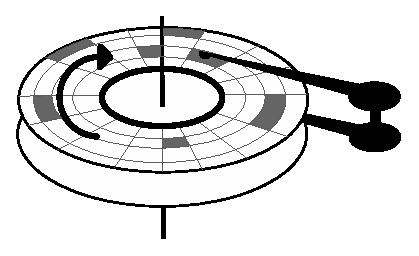
\includegraphics[width=\linewidth]{resources/made/external_storage_wblocks.eps}
                    \caption{External storage with the sectors to access highlighted}
                \end{figure}
            \end{block}
        \end{column}
    \end{columns}

    \framebreak{}

    \begin{itemize}
        \item In summary we can see the minimun, average and maximun time and write cost of each operation in a large B-Tree, using Big-O notation.
    \end{itemize}
    \begin{center}
        \begin{tabular}{@{}ccccccc}
            \toprule
                           & Retrival & \specialcell{Insertion without \\ overflow} & \specialcell{Insertion with \\ overflow} & \specialcell{Deletion \\ with or without \\ underfull} \\
                \midrule
                \multirow[c]{2}{*}{\(\Omega\)} 
                    & \(t = 1\) & \(t = h \) & \(t = h\) & \(t = h\) \\
                    & \(w = 0\) & \(w = 1\) & \(w = 1\) & \(w = 1\) \\
                \midrule
                \multirow[c]{2}{*}{\(\Theta\)} 
                    & \(t \leq h\) & \(t = h\) & \(t \leq h + 2 + \frac{2}{\alpha}\) & \(t \leq 3h - 2\) \\
                    & \(w = 0\) & \(w < 1 + \frac{2}{\alpha}\) & \(w \leq 3 + \frac{2}{\alpha}\) & \(w \leq 2h +1\) \\
                \midrule
                \multirow[c]{2}{*}{\(O\)}
                    & \(t = h\) & \(t = h\) & \(t = 3h - 2\) & \(t = 3h - 2\) \\
                    & \(w = 0\) & \(w = 2h + 1\) & \(w = 2h + 1\) & \(w = 2h + 1\) \\
            \toprule
        \end{tabular}
    \end{center}
    \begin{itemize}
        \item Where \(t\) is the number of fetch and readings of nodes on the secondary memory.
        \item And \(w\) is the number of writings of nodes on the secondary memory.~\parencite{bayer_organization_1972}.
    \end{itemize}\end{frame}


%\begin{frame}
%    \section{(a,b)-Tree}
%    \frametitle{(a,b)-Tree}
%\end{frame}
%\begin{frame}
%    \subsection{Properties}
%    \subsubsection{Keys and Sub-trees}
%    \frametitle{(a,b)-Tree Properties - Keys and Sub-trees}
%\end{frame}
%\begin{frame}
%    \subsubsection{Height}
%    \frametitle{(a,b)-Tree Properties - Height}
%\end{frame}
%\begin{frame}
%    \subsection{Structure}
%    \frametitle{(a,b)-Tree Properties - Structure}
%\end{frame}
%\begin{frame}
%    \subsection{Operations}
%    \frametitle{(a,b)-Tree Properties - Operations}
%\end{frame}

\begin{frame}[allowframebreaks,squeeze,allowdisplaybreaks]
    \section{Bibliography}
    \frametitle{Bibliography}
    \nocite{*}
    \printbibliography[heading=none]
\end{frame}

\end{document}
